\documentclass{ltjsbook}
\usepackage{docmute} 
\usepackage{../../myStyle} 

\begin{document}
\VerbatimFootnotes
\chapter{統計環境Rの導入}
\label{m03_introR}
ここまで，データを可視化したりデータの代表値を計算する方法について学んできましたが，実践上これらはすべてコンピュータを使って行います。
今回はPCを使った実践的な内容になります。パソコンを実際に触りながら，意図したことを正しく機械に伝え，意図した結果を得られるようにスキルアップしていきましょう。

\section{パソコンのファイル構造}
\subsection{パソコンの世界}
皆さんはパソコンをどういう用途で使うことが多いでしょうか。インターネットで調べ物をしたり\footnote{正確には，検索サイトを使って目的とするウェブサイトにアクセスする，という言い方になります。ウェブサイトを見る(ブラウズする)のはブラウザーというアプリケーションを使います。Chrome，Safari，Edge，Firefoxなどがブラウザーアプリケーションの名前で，Google，Yahooなど最初に開くウェブサイトのことをホームページと言います。ウェブサイトは個人や企業が提供しているものが多く，GoogleやYahooなどは検索サイトと言われます。}メールの読み書きをする，というのが多いかもしれません。FacebookやTwitter，InstagramなどSNSを利用する，これもインターネットに関係するアプリケーションですね。これらはスマートフォンやタブレットなどの方が手軽で便利にアクセスできるので，それらを使うことの方が多いかもしれません。

インターネットにアクセスするのではなく，手元のPCで(ローカル環境で)作業する例としては，文章を書くことが多いでしょう。大学生をはじめ研究者というのは基本的にコミュニケーションをする人ですから，半ば文筆業であると言っても過言ではありません。またこの文章を作成するために，必要な資料を作ることがあり，数値データを扱う場合は表計算ソフトを使うことになるでしょう。表計算ソフトの代表例として，Excel，Numbers，Calcsなどがあります。表計算ソフトは記述統計量やグラフの作成など，これまで学んできたことが簡単にできるものがありますが，それ以上の複数の変数を一度に扱った分析をするのには，機能的に不十分です。

そこで，より専門的な統計的処理をするためには，統計専用のソフトウェアを使うことになります。統計専用のソフトウェアとしては，SPSSやSAS，Stataなどの商用ソフトウェアもありますが，専修大学人間科学部心理学専攻では現在，Rを学科共通のツールとして利用することにしています。パソコンでこうしたソフトウェアを使うに先立って，重要な「ファイルの場所」について説明します。すでに情報の授業などで聞いたことがある話でしょうし，使い慣れている人にとっては当たり前の話なのですが，携帯電話端末やタブレットではファイルの位置がユーザに見えにくくなっていることも確かです。パソコンに苦手意識があったり，PCのトラブルに慣れていない人は今からのお話と，できれば付録(付録\ref{computer})も併せて目を通しておいてください。

\subsection{ファイルの場所}
\label{filelocale}
パソコンを使うにあたって話をしておかなければならないのは，まず「ファイル」という考え方です。
パソコンをはじめ，スマホやタブレットなどコンピュータ，あるいは万能計算機は，いろいろな機能を有しています。文字を書いたり数字を計算したり，音楽を鳴らしたり映像を加工したり，ですが，これらはすべて0/1というデジタルなデータであり，文字，数字，音，画像，動画などすべて0/1というデータに規格化したことが\textbf{情報化社会}の本質です。その中身が何であれ，データのまとまりのことをファイルと言います。

アプリケーションを実行するのもファイルですし，データを保存しておくのもファイルです。パソコンが機能するのに必要なファイルは非常にたくさんあるので，整理するためにディレクトリ(フォルダ)の中にまとめて，階層構造を持って保存されています。複数のファイルはフォルダにまとめますが，フォルダをまとめたフォルダ，というように「階層構造」をつくっています。
図\ref{fig::02_02}や\ref{fig::02_03}に，WindowsやMacでファイルを見るための画面(アプリケーション名がそれぞれエクスプローラ，ファインダーと異なります)を示しています。いずれもアイコンの色や形は違いますが，フォルダの中にフォルダやファイルが含まれる，という形になっているのがわかると思います。

\begin{figure}[ht]
    \centering
    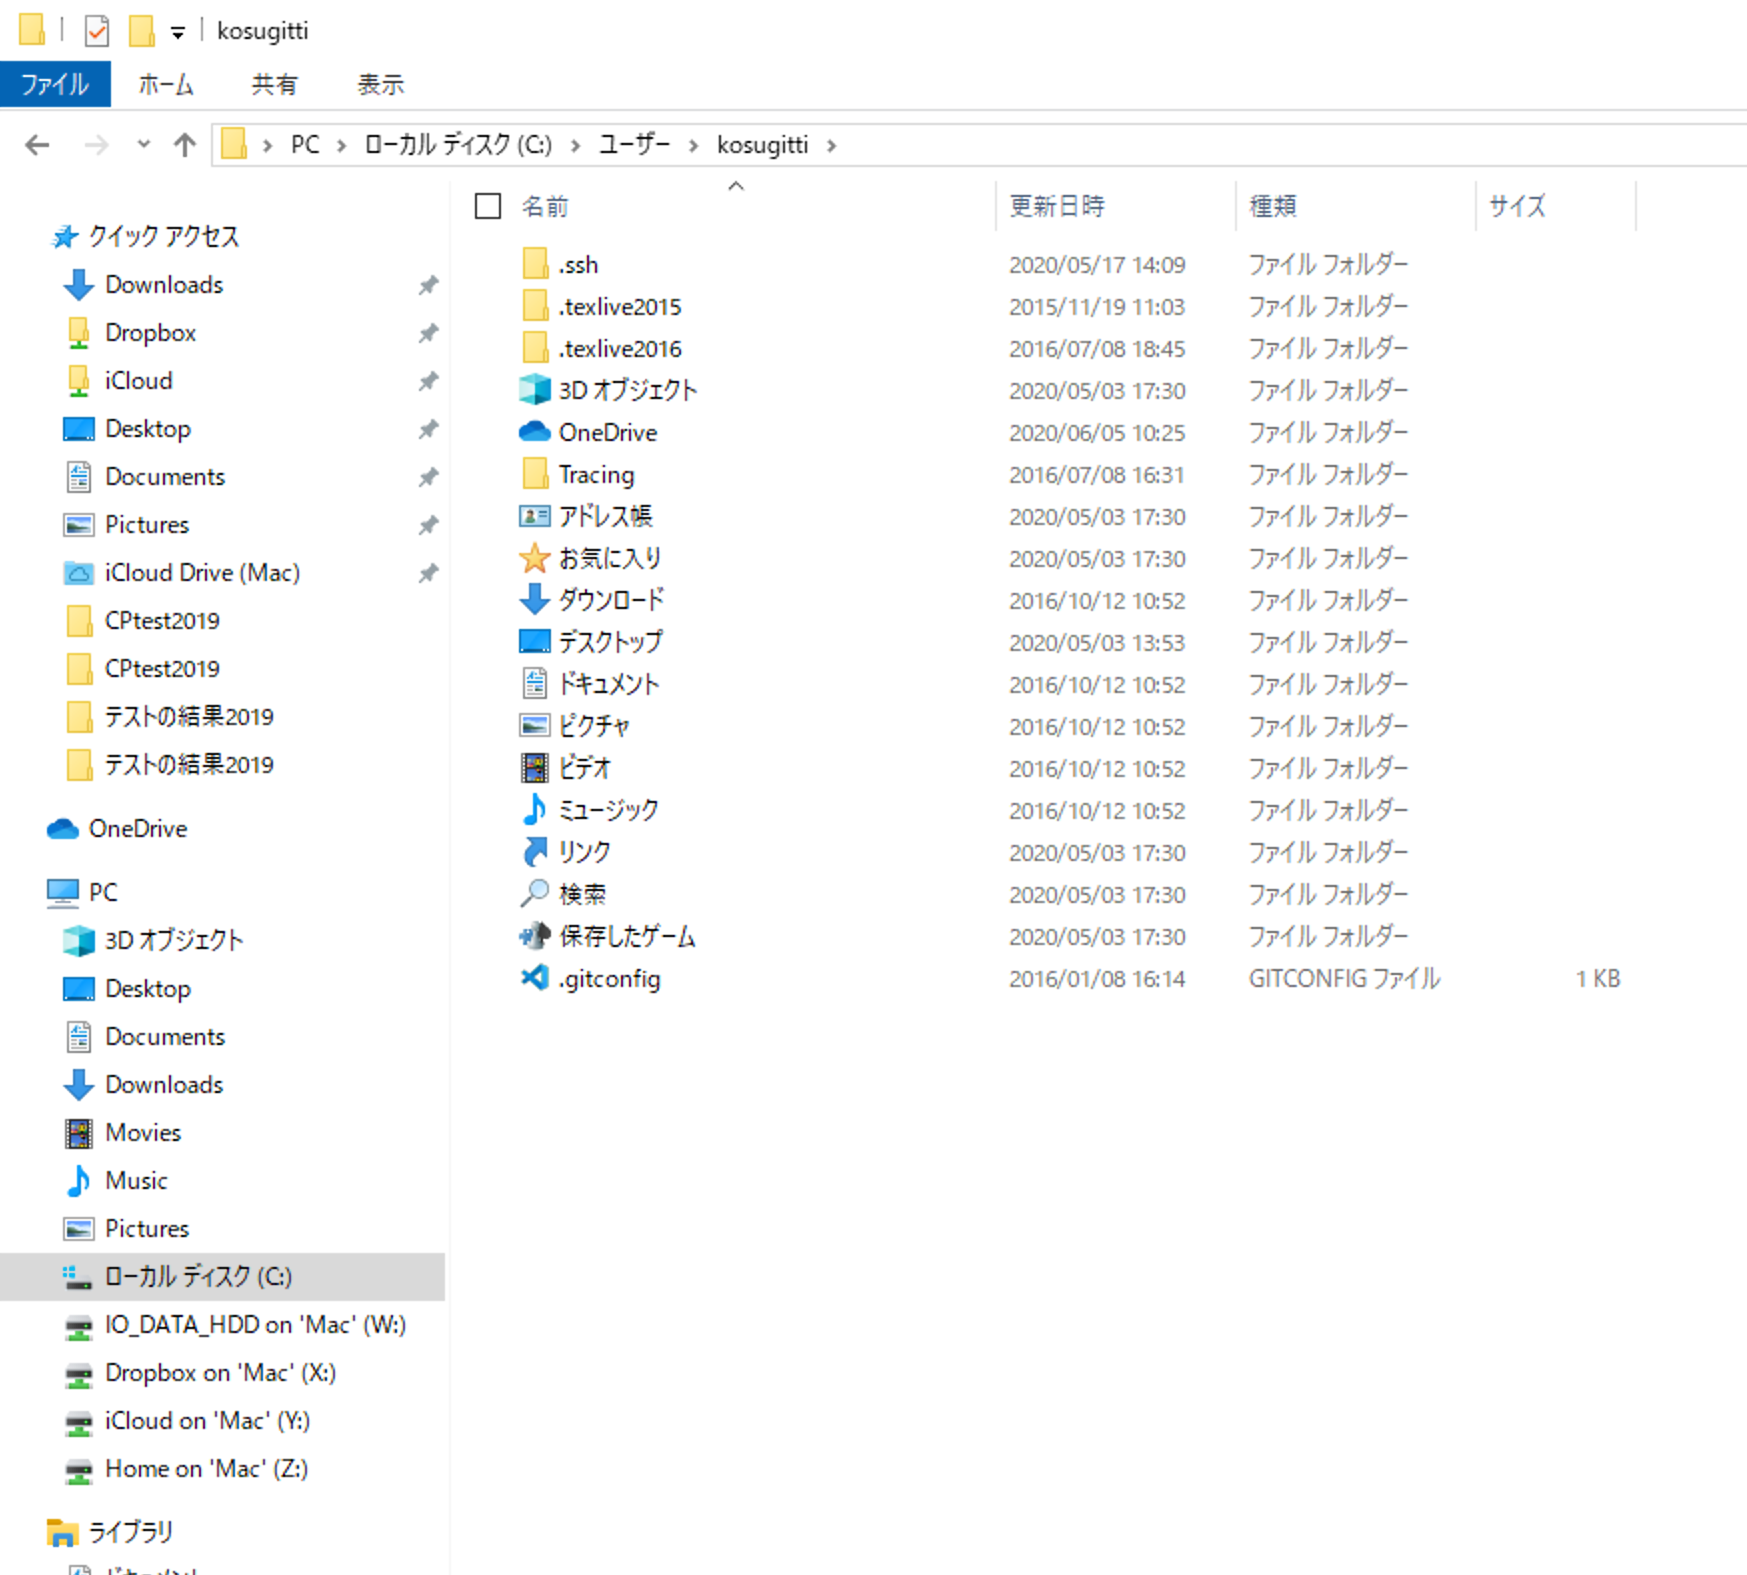
\includegraphics[keepaspectratio,width=0.8\linewidth]{../images/03_introR/computer_02.png}
    \caption{Windowsのエクスプローラ画面}
    \label{fig::02_02}
\end{figure}

\begin{figure}[ht]
    \centering
    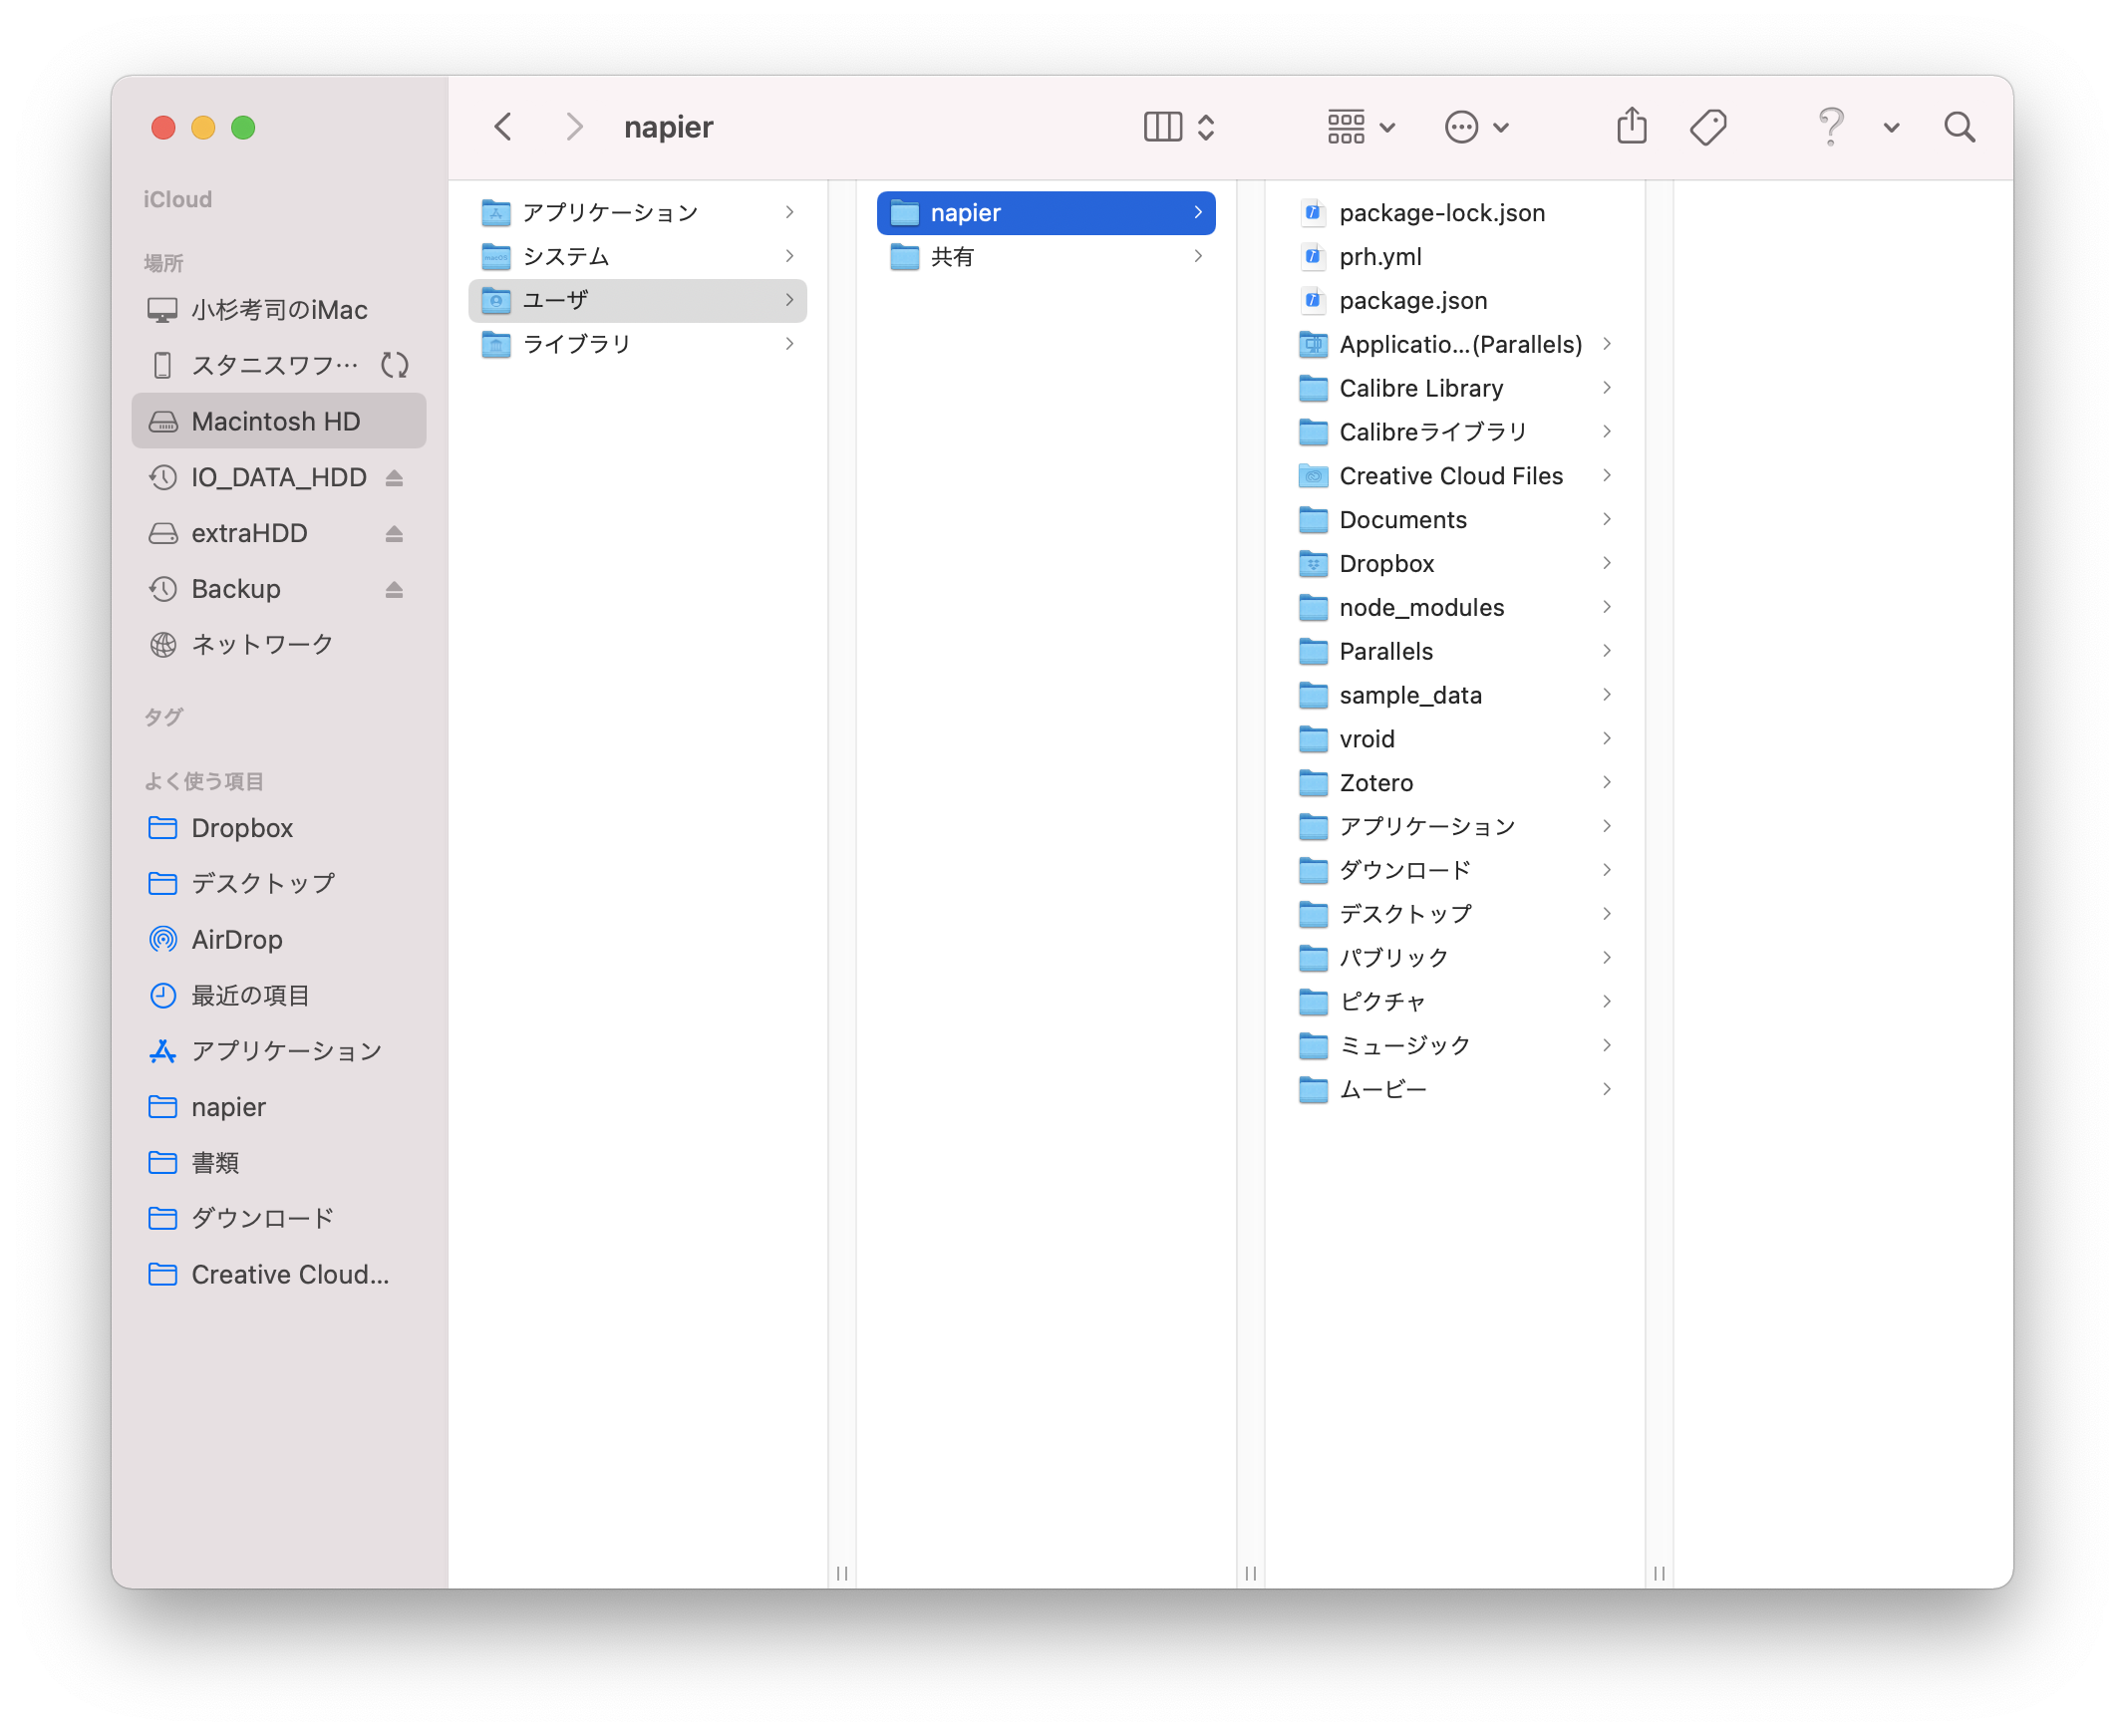
\includegraphics[keepaspectratio,width=0.8\linewidth]{../images/03_introR/computer_03.png}
    \caption{Mac OSのファインダー画面}
    \label{fig::02_03}
\end{figure}

ここでWindowsの画面にある，エクスプローラの上部を見てみましょう。この例では「PC>ローカルディスク(C:)>ユーザー＞kosugitti>」とありますね。日本語の文字が入っているので2バイト文字なのかと思いきや，ここをクリックしてみると「C:¥Users¥kosugitti」と出てきます。実はこちらが本当の名前で，ローカルディスクとかユーザーと表示されていたのは使い手に優しく表現しているだけのイリュージョンなのです。ここでC:とあるのはドライブと呼ばれ\footnote{なんでCから始まってて，AやBじゃないんだ，と思われるかもしれませんが，これにも歴史的経緯があります。かつてのパソコンは，フロッピーディスクドライブ(FDD)が2器ついているのが基本で，それらにA,Bと割り振られていました。その後に出てきた内蔵ハードディスクドライブはCとするのが順当だったわけです。その後FDDは時代とともに使われなくなりドライブも無くなったのですが，ドライブレター(ドライブに割り当てた文字)は残ったのです。}，記憶装置の実体を指します。この場合はパソコンに内蔵されたハードディスクドライブです\footnote{ハードディスクドライブ(HDD)とは，FDDの中に入っている磁気媒体の円盤が積み重なったもので，FDDよりも大容量のデータを保管できます。FDDが1MBぐらいであるのに対し，HDDは数TBのものが現在主流です。}。このCドライブの中に，Usersというフォルダがあり，その中にkosugittiというユーザが使う領域がある，という区分になっています\footnote{最初にパソコンを購入した時に，このパソコンで使うユーザの名前は何ですかと聞かれると思います。その時に入力したものがユーザ名になりますが，その時に2バイト文字でユーザ名を入力していると，その後のアプリケーションがうまく動かないエラーが出てくることになったりします。}。
\begin{figure}[ht]
    \centering
    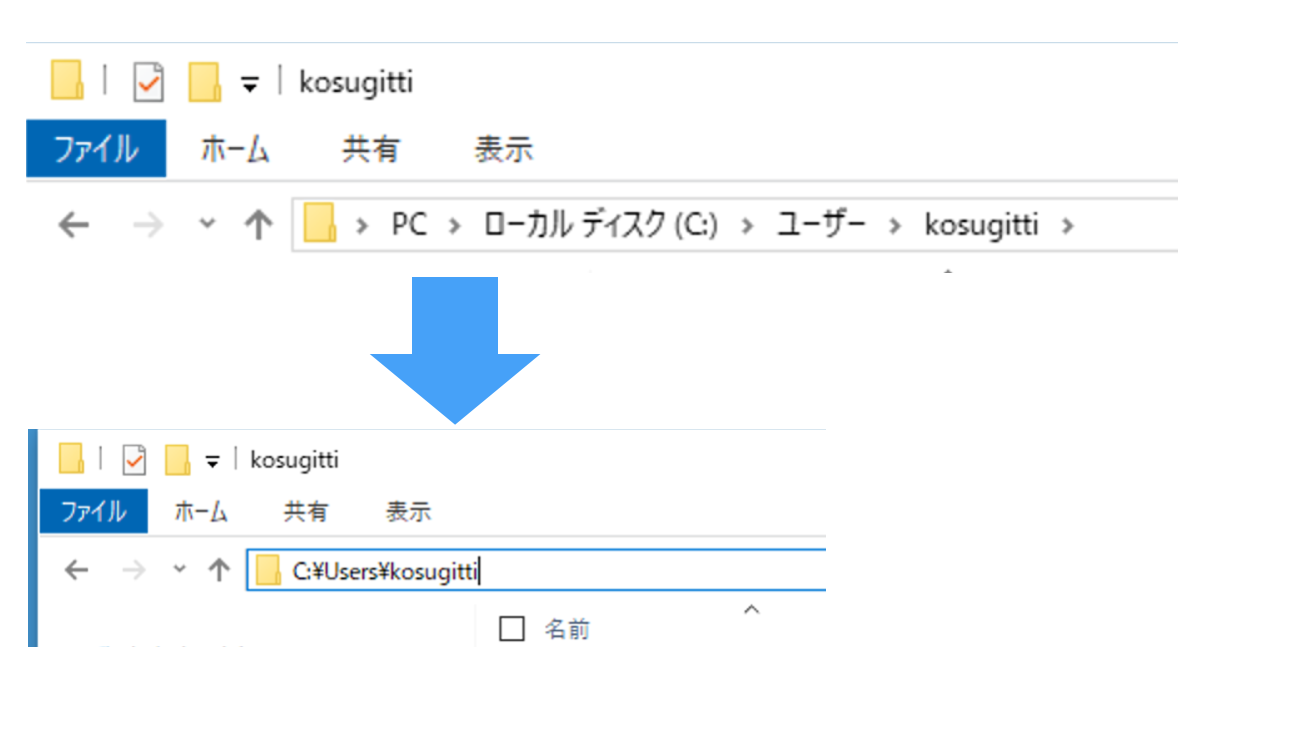
\includegraphics[keepaspectratio,width=0.8\linewidth]{../images/03_introR/computer_04.png}
    \caption{Windowsのフォルダ階層}
    \label{fig::02_04}
\end{figure}
図\ref{fig::02_05}にはMacの画面を示していますが，ここでもドライブ，フォルダ，フォルダ，という構造になっていること，ユーザのなかにnapierというユーザ名があることなどが確認できると思います。Ubuntuなど別のOSでもこうした仕組みは同じです。これらの画面を見ながら自分で使うファイル，作ったファイルがどこにあるのかをはっきり把握できるようにしておいてください。
\begin{figure}[ht]
    \centering
    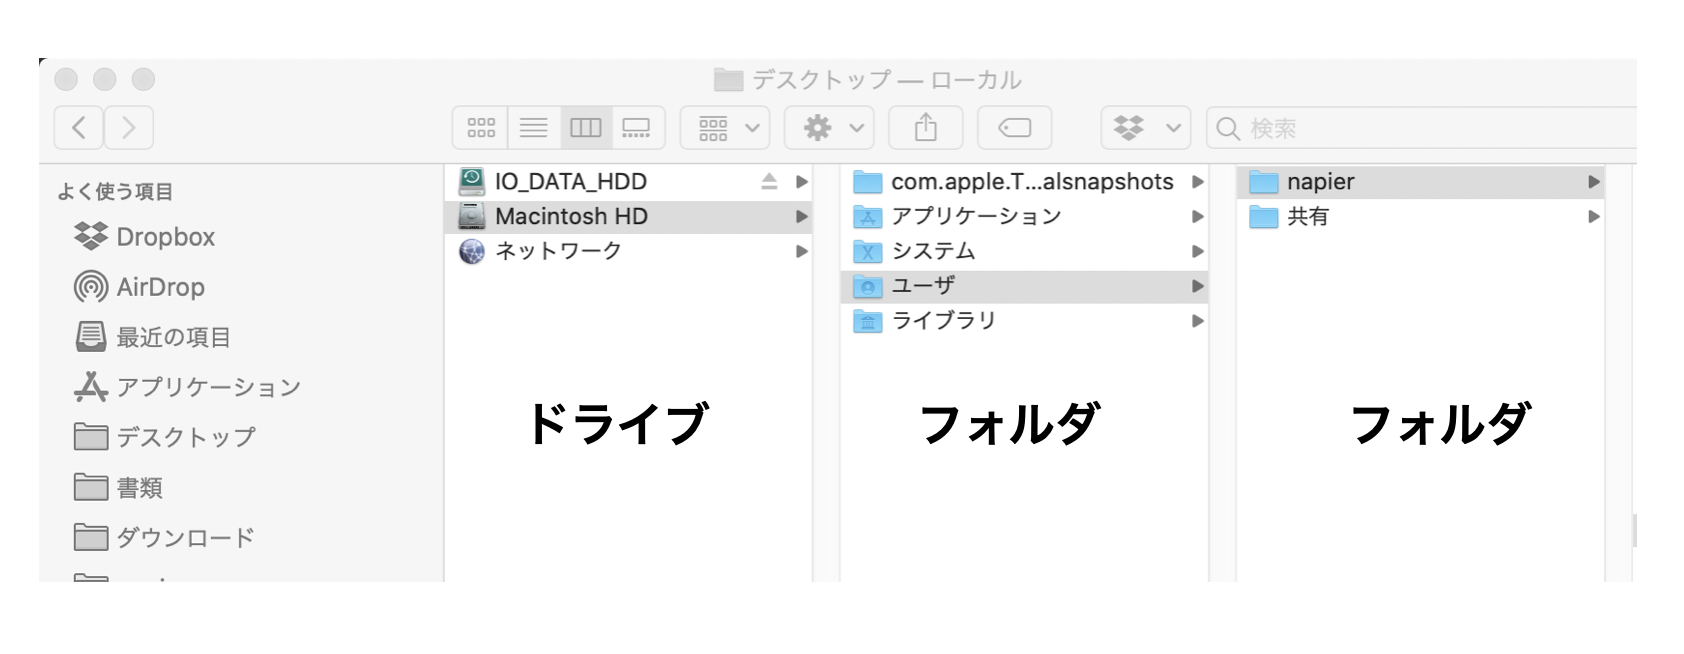
\includegraphics[keepaspectratio,width=0.8\linewidth]{../images/03_introR/computer_05.png}
    \caption{Mac OSのフォルダ階層}
    \label{fig::02_05}
\end{figure}

これからの大学生活で，皆さんはいろいろな授業でレポートを書いたり，統計計算をしたりします。
それらを「書類」というフォルダの中にまとめて入れてしまうと，後で探す時に大変ですから，授業ごと，あるいは研究テーマごとなどにフォルダを作り管理するようにしてください。
この授業でも，よく相談されるエラーが「ファイルがありません」というものです。作ったはずのものがない，保存したはずのものがない，というトラブルの原因はほぼ確実にユーザの責任で，置いた場所がわからなくなっているのです。これについては相談されても「自分で思い出してください」としか言えませんので，ファイルの整理整頓を常に心がけてくださいね。

\section{統計環境R/RStudioの準備}
それではやっと本質，パソコンを使っていくことにしましょう。とくにここでは統計環境\keytermL{R}{R}について解説します。

Rは統計環境，統計言語とも呼ばれることがあります。統計に関する分析をCUIで行うので統計``言語''と呼んだり，数字だけでなく図を描くなど数値処理に関わることを全体的にカバーしているので``環境''と呼ばれたりします。Rが優れている点はフリーソフトウェアであるという点で，誰でも無償で利用できることです。商用ソフトウェアと違って，ソースが公開されているのでその気になれば誰でもその内部構造を調べることができますから，間違い(エラー，バグ)がないかどうかをみんなの目でチェックできるというのが利点です。金銭的に補償があるわけではないのですが，そもそも学問の世界は市井の資本主義的発想とは異なる価値で評価される世界ですから，無償であることは問題になりません。

またRは多くの研究者が利用しており，その研究成果をフリーソフトウェアの精神で共有しています。こうしたRの基本関数以外の機能は，パッケージという形で提供されます。Rのパッケージを共有している場所はThe Comprehensive R Archive Network(\keytermL{CRAN}{CRAN})と呼ばれ，ここに登録されているパッケージは誰でも利用できます。最先端の分析ツールがここを介して共有され，間違いや問題が生じたら随時修正されていきますので，成長する統計ソフトウェアということができるでしょう。

またこの授業では，Rを使うにあたって\keytermL{RStudio}{RStudio}という総合開発環境アプリを使います。Rというアプリケーションを便利に使うためのアプリケーション，それがRStudioです。

Rは優れた統計ツールではありますが，本体だけでは簡素な言語的やりとりができるに過ぎません。分析を進めていくとすぐにわかりますが，ファイルの操作や描画機能，過去ログの参照や管理など，統計言語を扱う際にそれを取り巻くさまざまな操作が必要になります。ここをカバーしてくれるのがRStudioというアプリケーションなのです。

RStudioはそれ単体では使うことができません。Rが入っているPC上で，Rを取り込んで初めて意味のあるアプリケーションになります。Rの計算機能を活用するだけでなく，文書作成機能やデータベースとの連携など非常に高機能な統合的サービスを提供してくれます。文章を書き，その文章に必要な計算を行い，その結果がすべて記録(スクリプト，コマンド，プログラム)として残るわけですから，科学論文を書くためにはRStudioだけでも十分です。


\subsection{環境を構築しよう}
専修大学の情報科学センターにあるPC室や，心理学科が管理する4号館4FのPC室にはRやRStudioがすでにセットアップされていますので，これを利用するのであればとくに準備は必要ありません\footnote{他にも心理学科には，計算機サーバというのがあり，ここにRStudio Serverが準備されています。RStudioServerは，インターネットを介するウェブブラウザからRStudioにアクセスすることができるものです。残念ながらまだ試験的導入段階で，心理学科の学生が一気にアクセスするとサーバがダウンしてしまいますので，希望者のみの利用にとどまっています。}。

しかしながら，大学のPC室に行かなくても自宅で論文やレポートを書きたい，ということもあるかもしれません。また，大学などの設備は大学が管理していますので，自分でパッケージを追加したい，とおもっても管理権限がなくうまく行かないこともあるかもしれません。幸いRやRStudioはフリーソフトウェアですので，手元のPCにインストールして環境を構築するにしても，元手は一切かかりません。これを機に，自分のパソコン環境にR/RStudioを準備しておくと良いでしょう。

RやRStudioの環境構築については，その方法を検索すればさまざまなものが出てきますので，そちらを参考にしてください\footnote{Rの唯一の弱点は検索可能性が低いこと。Rという一文字で検索してもまともなものにヒットしないので，``CRAN''とか``RとRStudio インストール''など周りに言葉を足して検索してみてください。}。新しいものでは，高知工科大学柳内先生のサイト\footnote{\url{http://yukiyanai.GitHub.io/jp/resources/}}とか，
Syunsuke Fukuda先生の初心者向けRのインストールガイド\footnote{\url{https://syunsuke.GitHub.io/r_install_guide_for_beginners/}}などは網羅的かつ丁寧なので，よく読んで始めると良いでしょう。Quiitaというエンジニアがよく参照するブログの記事\footnote{\url{https://bit.ly/3MfK3SD}}なども良いと思います。書籍では，手前味噌で恐縮ですが\citet{kosugi2019}などが良いでしょう\footnote{なお，インストールに際しては，RStudio DesktopのFree editionを選んでください。RStudio CloudやRStudio Serverは別のものです。}。

以降は環境が準備できているものとして解説を続けます\footnote{トラブルがあって環境の準備がうまくできていない場合は，\texttt{classkosugitti@gmail.com}までご相談ください。}。

\section{R/RStudioの基本操作}
それでは今から，RStudioを使った統計処理の演習を始めましょう。少し不便かもしれませんが，この資料を見ながら，\textbf{必ず自分でコードを入力しながら}進めていってください。テキストと同じ結果が手元で再現できることを確認しながら進むことは，再現できることの重要性の確認になります。また，最初のうちは打ち間違えなどで思うように動かないことも頻発するでしょうが，その経験を繰り返すことで徐々に使い慣れていきます。失敗の経験はテキストの文中に書き込まれていませんから，読むだけでは身につきません。また，読み進んで気が向いたところだけ実行するときは，その前のデータや内容を参照している場合にエラーになるので，結局元に戻ってやり直すことになります。最初のうちは写経して作法を身につけることも重要なのです。最初の基礎的な訓練\footnote{キーボードの入力に慣れていない人は，ブラインドタッチの練習をすることをお勧めします。キー入力は今後も活用できる社会人の基本スキルですので，なるべく早く習得しておいた方が人生が楽しくなります。ブラインドタッチの練習には，寿司打などのサイト\url{http://typingx0.net/sushida/play.html}で遊びながら学べていいですよ。ちなみに今やってみたら，私の成績は「高級10,000円コース【普通】で、★5,820円分 お得でした!（速度：6.1key/秒、ミス：57key」でした。}ができていると，徐々に大きなプロジェクト\footnote{卒論は4年間の集大成になる個人プロジェクトです。}を動かすことができるようになりますので頑張って！

\subsection{RStudioの機能と画面}
最初にRStudioを起動すると，図\ref{fig::05_01}のような画面になっていると思います\footnote{こちらはMacOS11.1，RStudioは1.4.1103，Rは4.0.3の環境で行っています(執筆時2021年2月2日)。OSが違うとか，バージョンが違う，サーバ版を使っているとかで細部が異なっている可能性があります。}。ここでメニューから\verb| File > NewFile > RScript |と進むと(図\ref{fig::05_02})，画面に白いページの領域が追加されます(図\ref{fig::05_03})。

大きくみると画面が四分割されたようになります。この4つの領域を基本として話を進めていきます\footnote{RStudio version1.4から，列を追加することができるようになりましたので，必ずしも四分割で使わなければならないというわけではありません。どこに何があるのかを把握していればOKです。ちなみに列を増やしたり配置を変えたりするのは，\verb|Tool > Global Option > Pane Layout|から可能です。}。

\begin{figure}[ht]
    \centering
    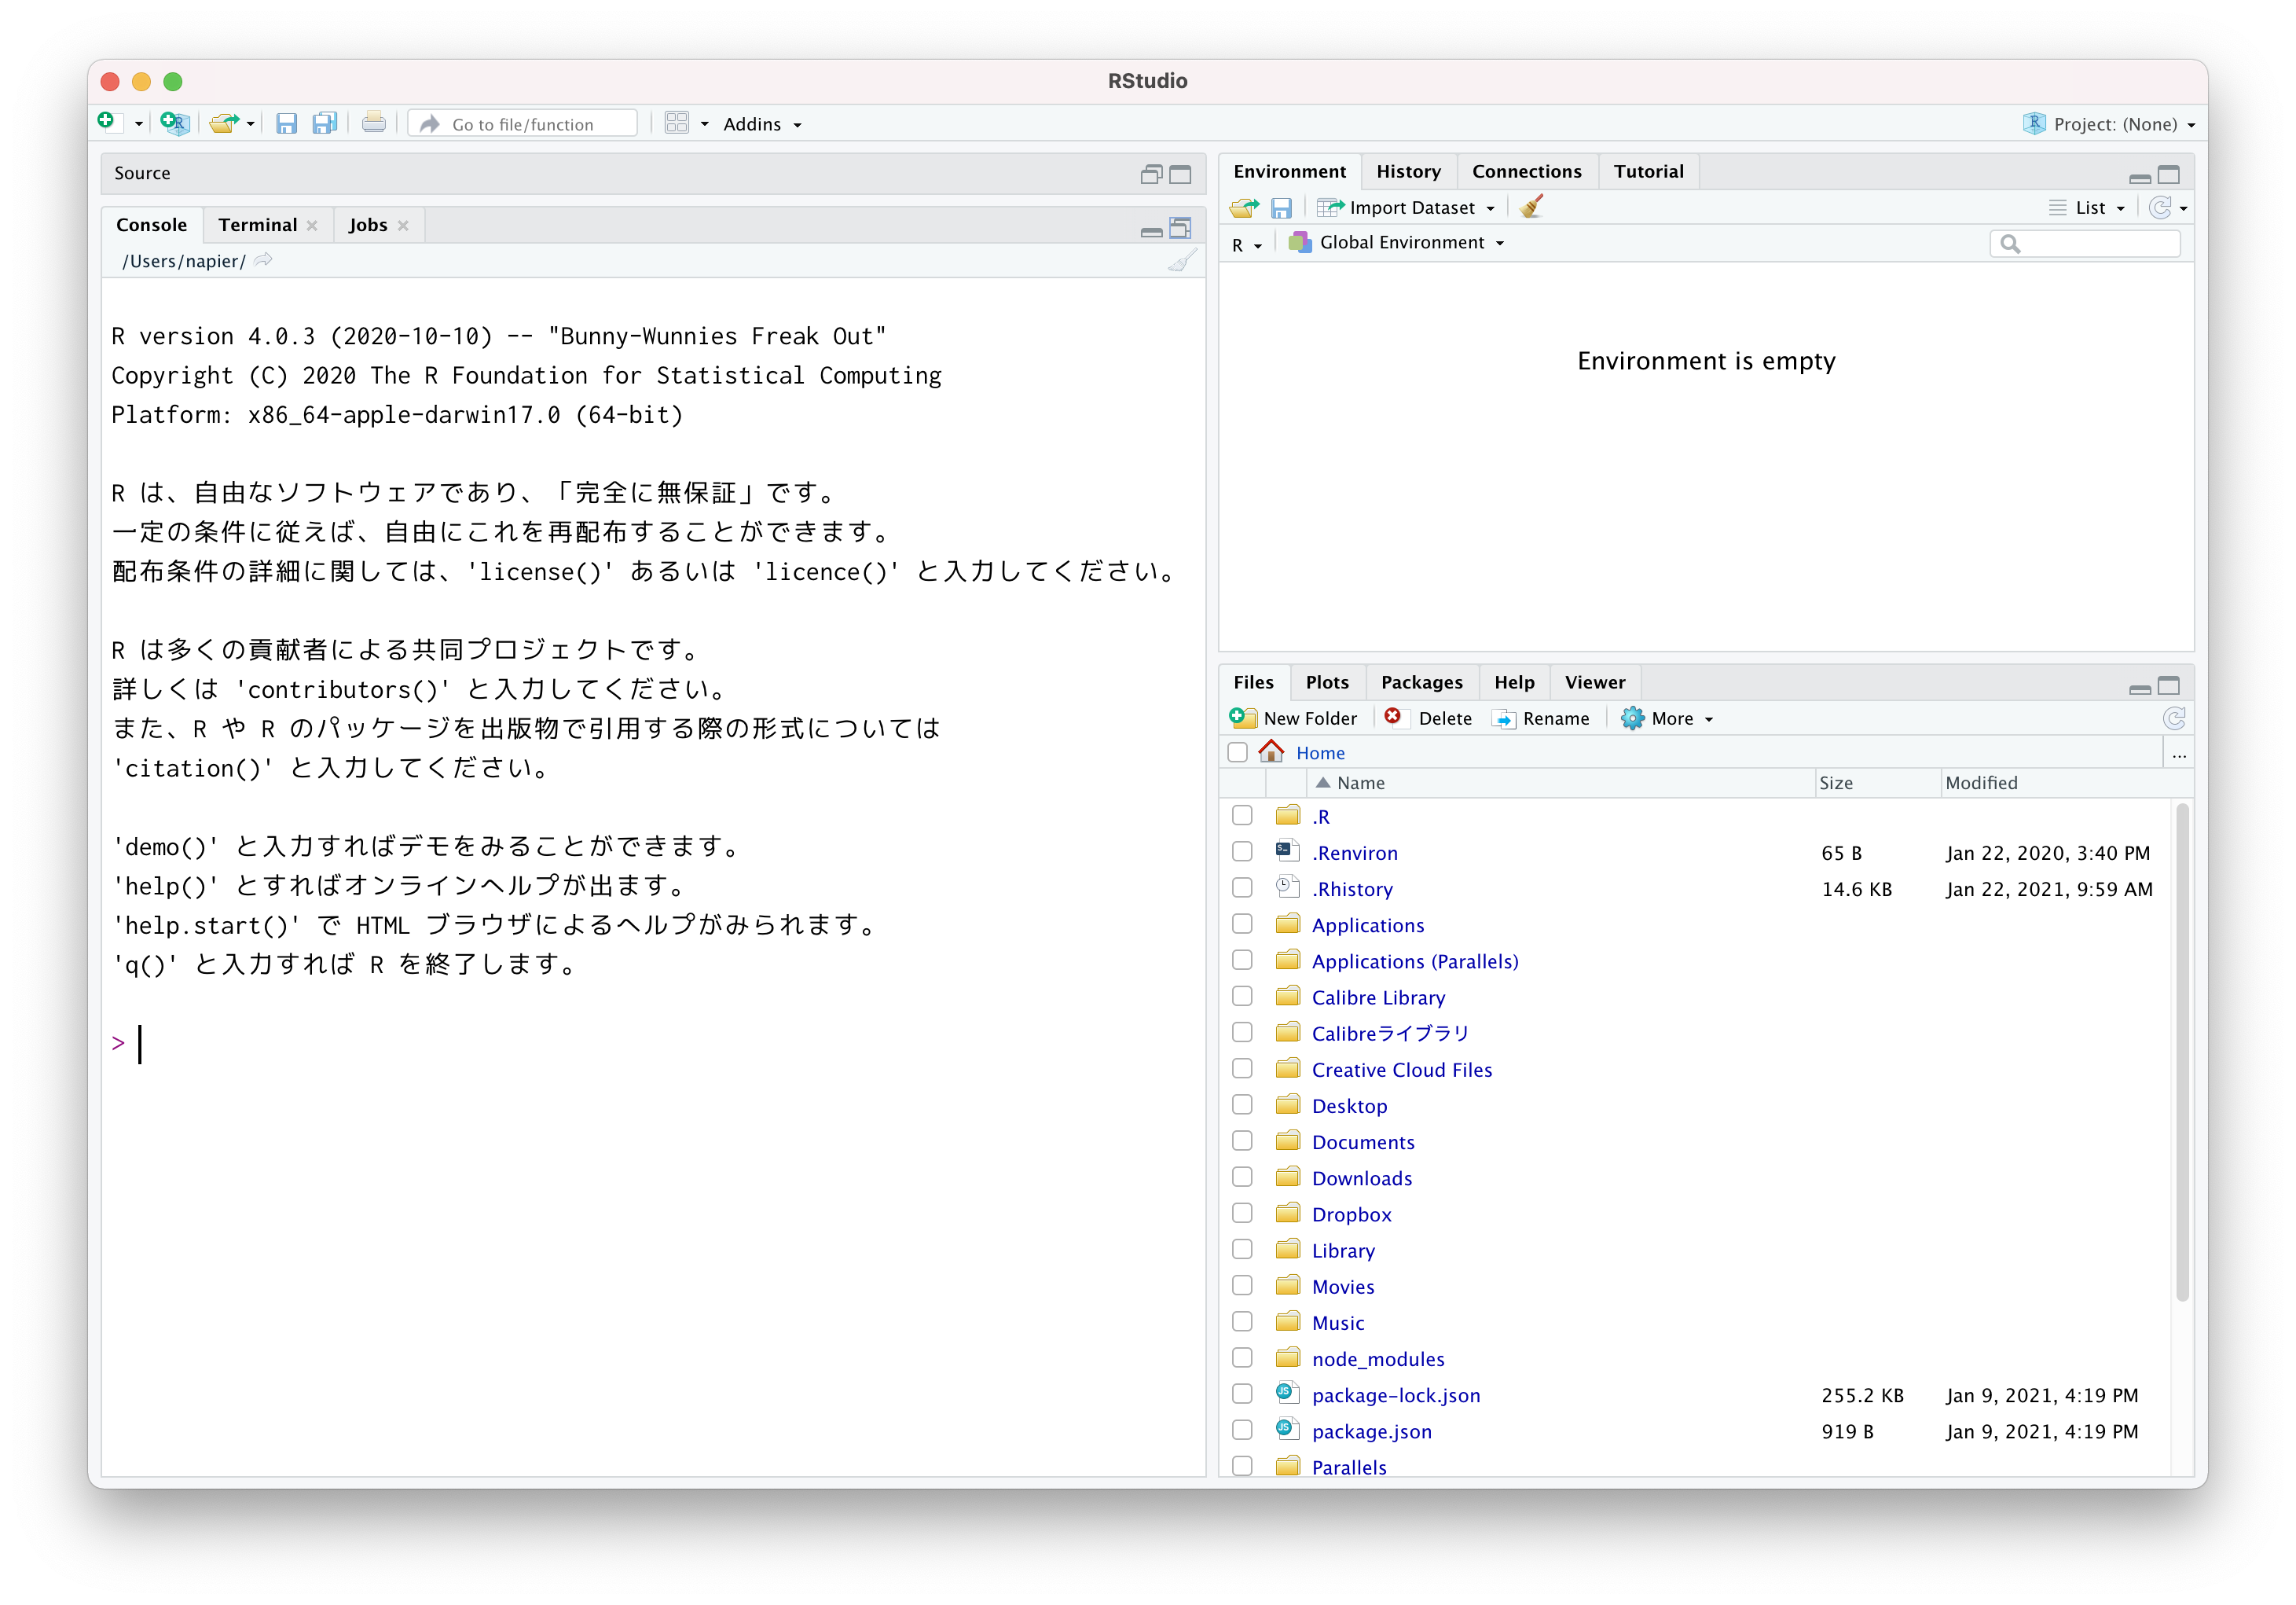
\includegraphics[keepaspectratio,width=0.75\linewidth]{../images/03_introR/Screen1.png}
    \caption{RStudio起動初期の画面}
    \label{fig::05_01}
\end{figure}

\begin{figure}[ht]
    \centering
    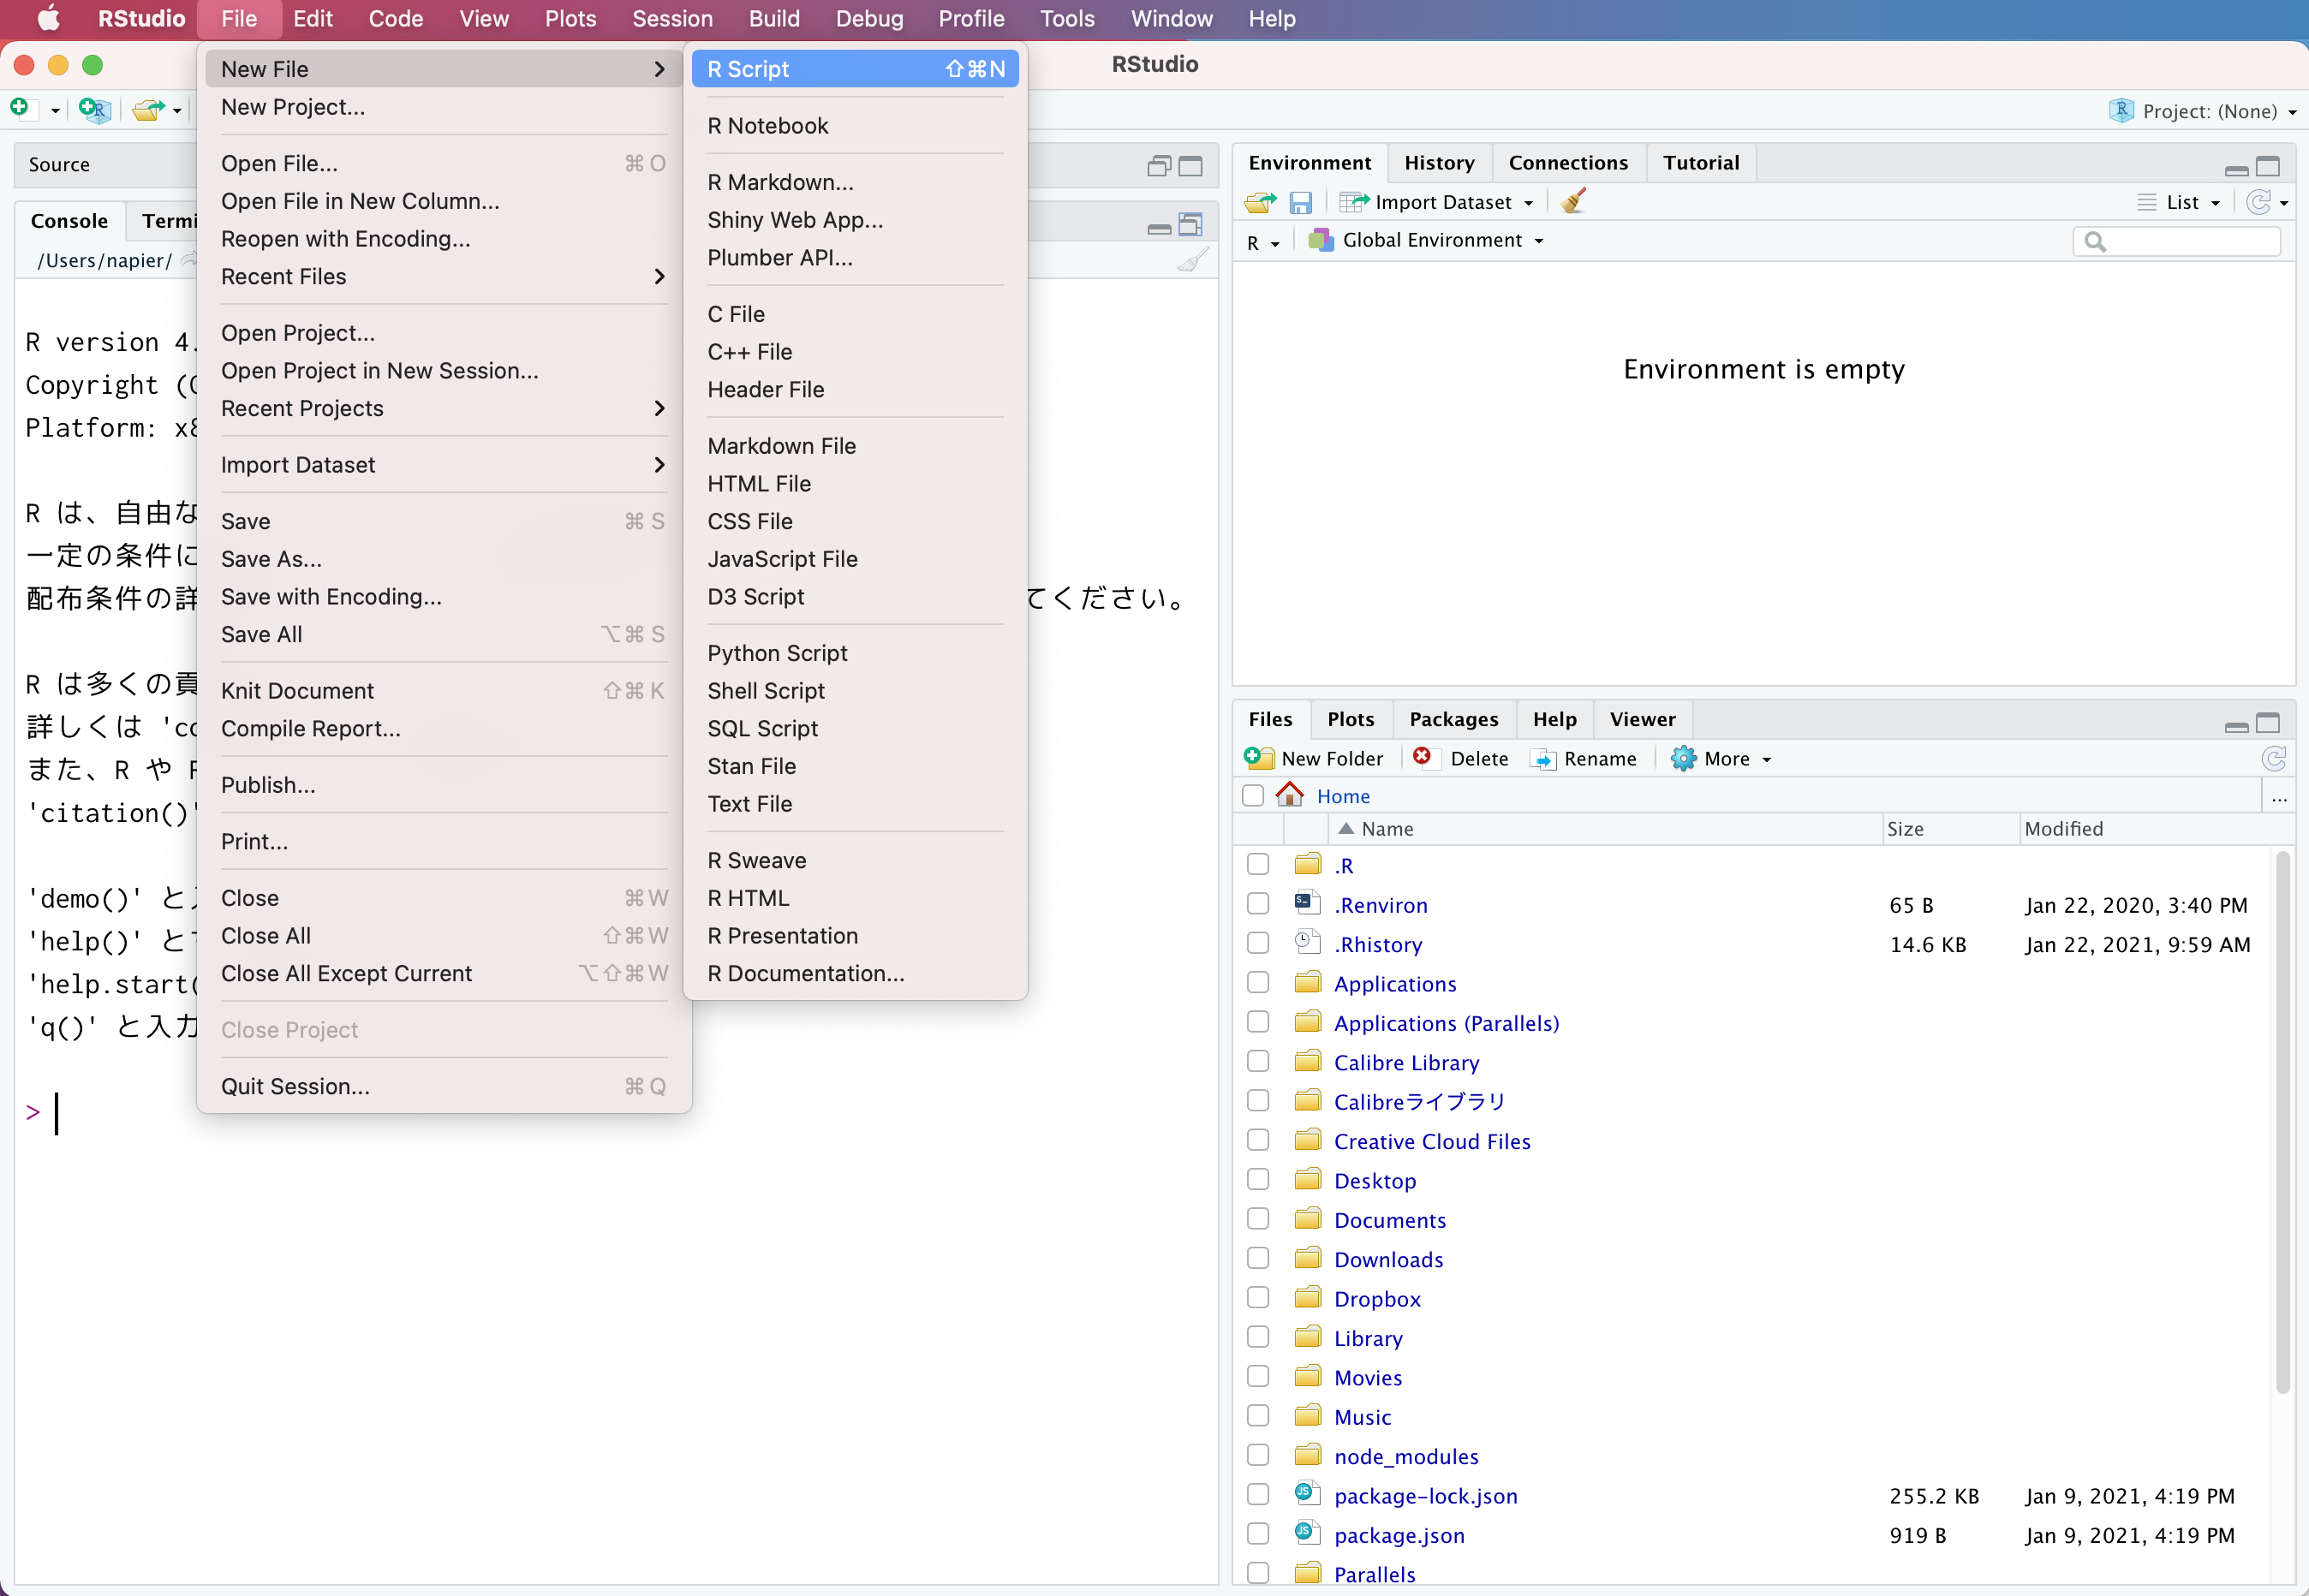
\includegraphics[keepaspectratio,width=0.75\linewidth]{../images/03_introR/Screen2.png}
    \caption{新しくスクリプトファイルを開く}
    \label{fig::05_02}
\end{figure}

\begin{figure}[ht]
    \centering
    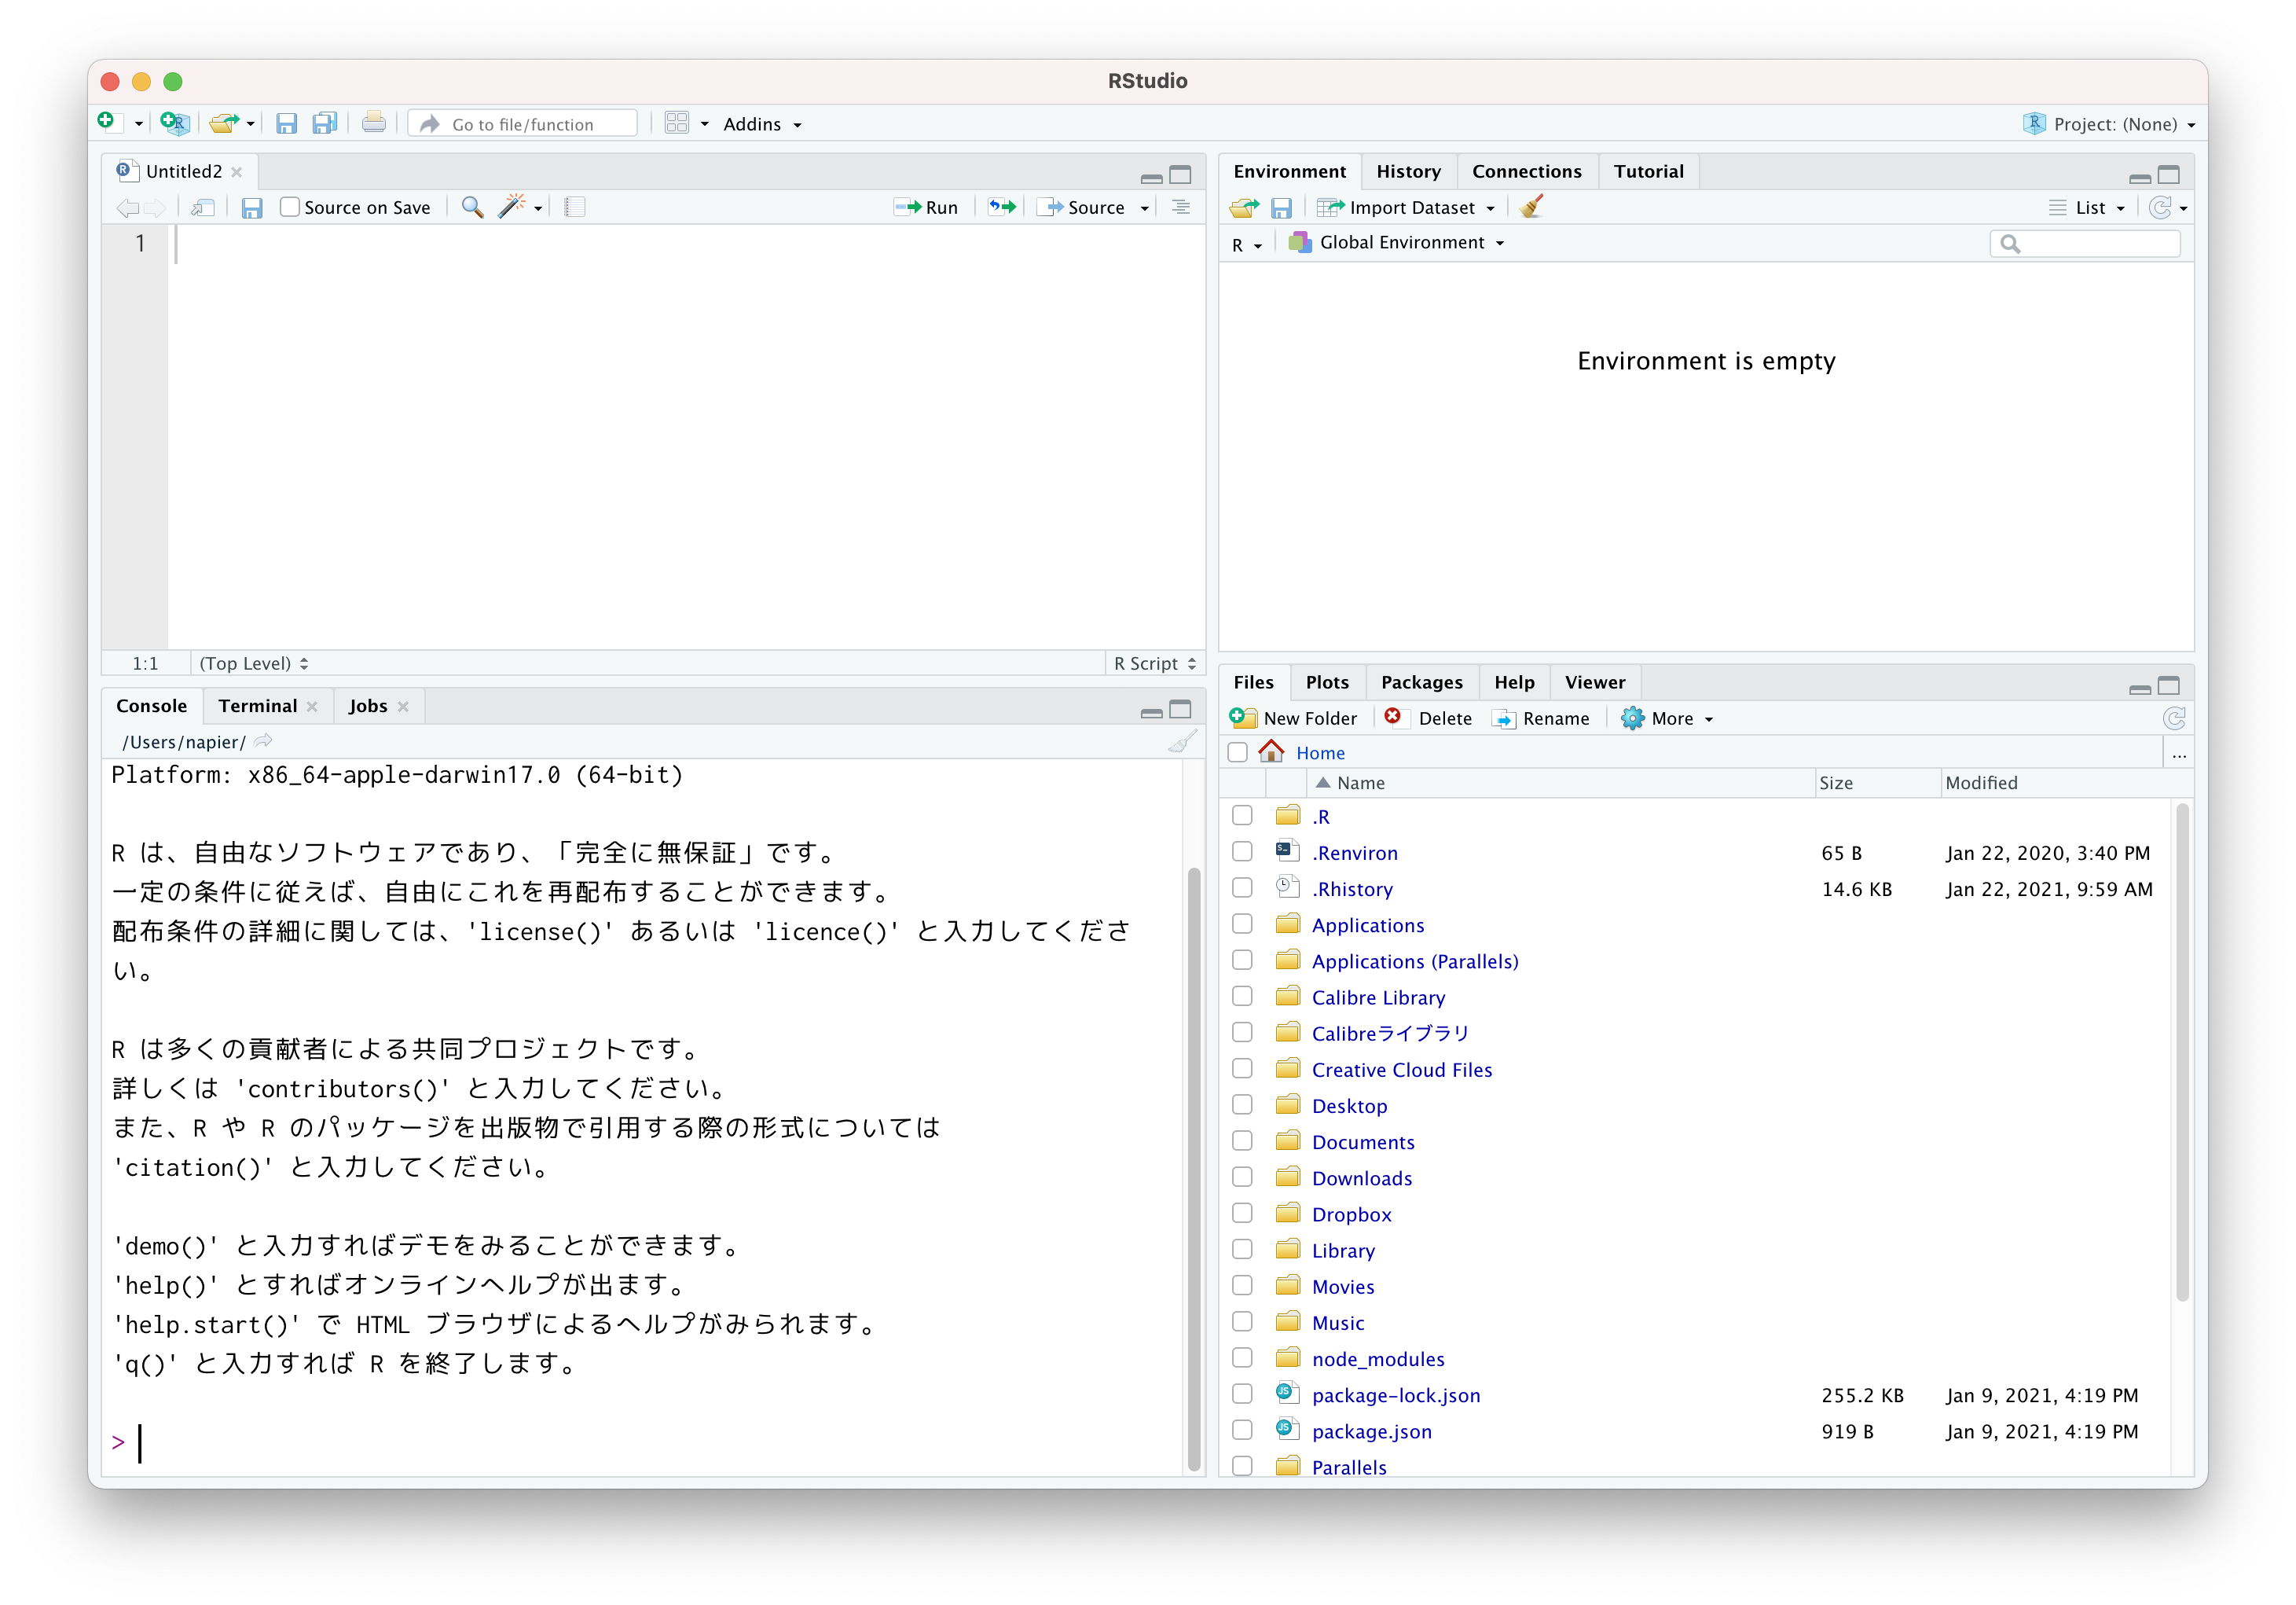
\includegraphics[keepaspectratio,width=0.75\linewidth]{../images/03_introR/Screen3.png}
    \caption{RStudioの画面}
    \label{fig::05_03}
\end{figure}

\paragraph{コンソール・ペイン}
デフォルトでは画面の左下になりますが，\keyterm{コンソール}{こんそーる}{Rの出力}ペインにあるのがRそのものです。
RStudioはRを取り込んで使いやすくする環境を提供するもの，という話をしましたが，とりこまれたRだけの画面が左下にあります。そこにはRのバージョン情報や，次のような注意書きが書かれています。
\begin{Rscreen}{}{}
    \begin{verbatim}
	R version 4.0.3 (2020-10-10) -- "Bunny-Wunnies Freak Out"
	Copyright (C) 2020 The R Foundation for Statistical Computing
	Platform: x86_64-apple-darwin17.0 (64-bit)

	R は、自由なソフトウェアであり、「完全に無保証」です。
	一定の条件に従えば、自由にこれを再配布できます。
	配布条件の詳細に関しては、'license()' あるいは 'licence()' と入力してください。
	\end{verbatim}
\end{Rscreen}

その下に\texttt{>}という記号が出ていると思います。これは入力を待っている状態でこの記号の左側に命令をどうぞ，という意味です。この記号が出ているときは，Rは次の動作準備OKで指示を待っているという状態です。ここにコードを入力すれば計算結果が出力されるのですが，その前にスクリプトペインの説明をします。
\paragraph{スクリプト・ペイン}
スクリプトペインは，Rのコードを書くところです。Rは一問一答型(インタプリタ\footnote{プログラミング言語の実行方法として，コードを逐次翻訳していく方法と，プログラム全体を一気に機械語に翻訳して実行する方法のに種類があります。前者をインタプリタ方式，後者をコンパイラ方式と言います。インタプリタ方式の利点は書いたコードがすぐに実行されるので，どこでどういう処理がされているか分かり易いことです。エラーがあってもすぐにその場で帰ってきます。コンパイラ方式の利点は実行速度です。全部の処理を一気に機械語に翻訳してあるので，計算速度が非常に早くなります。コンパイラ方式の欠点は，どこでエラーが生じたかわかりにくい点です。}方式ともいいます)なのですが，実際の統計処理はあれをして，これをして...とたくさんの処理が連なることになります。この一連の手続きを書いておくのがこの場所です。

スクリプトとはお料理のレシピのようなものです。1つ1つの計算は，たとえば「玉ねぎをみじん切りにする」といった単一の作業をさせることになりますが，全体としてハンバーグを作るのが目的であれば，1つ1つの作業をすべて順番通りに実行しなければなりません。直接コンソールペインに書き込んで言ってもいいのですが，途中で「今どの工程だっけ」というのがわからなくならないとも限りませんので，いったんスクリプトのところに書いてから実行する，という手段を取るのが便利です。

実際にコマンドを1つ1つ書いていくときには，書き間違えたり違う方法を試したくなったりするので，書いたり消したりしながら進むのが普通です。ですが最終的には清書したものだけを残すようにしましょう。下書きの要素もすべて記録していると，あとで何がどうなったかわからなくなります。また，何度か繰り返しているうちに「何にどのような操作をしたか」がわかっているようでわからなくなることがあります。最終的には，1つのスクリプトファイルを一行目から順に実行していけば，すべての作業が再現できるようにする，ということが重要です。途中で別のレシピを参照したり，記録されていない操作を挟むのはやめましょう。

さてでは，このスクリプトペインに\texttt{code:\ref{code:05_01}}を書いてみてださい\footnote{この資料では指示がわかりやすくなるように行番号を含めて表示していますが，実際は行番号を入力する必要はありません。}。

\begin{lstlisting}[language=c++,label={code:05_01},caption={四則演算のコード}]
	# 四則演算
	1+2
	2-4
	3*5
	6/3
	sqrt(16)
\end{lstlisting}

\paragraph{コード解説}
\begin{description}
    \item[1行目] コメントアウト。\verb|#|記号で始まる行は，その後ろに何を書かれていてもRは無視します。なので，この記号を冒頭に描いて，ここに何をしているかという説明を書き入れています。このコメントは，あとで見直す時に何をしていたか判るためのものなので，必ず書かなければならないというものではないのですが，あればあるほど親切で丁寧なコードと言えるでしょう。
    \item[2-5行目] 順に和，差，積、商を求めるコードです。積\verb|*|と商\verb|/|の記号はPCではこのように書きますので注意してください。
    \item[6行目] これは関数を使って答えを出しています。\texttt{sqrt}関数は正の平方根を返します。
\end{description}

書いたあと，スクリプトペインの右上にある\texttt{Run}を押すと一行ずつ実行されていきます。あるいは，CTRL+Enterでもスクリプトをコンソールに送り込むことができます。マウスで複数行を選んで\texttt{Run}ボタンを押すと囲んだ箇所を実行することもできます。このスクリプトペイン全体を実行したいときは\texttt{Source}ボタンを押します。
\begin{figure}[ht]
    \centering
    
\includegraphics[keepaspectratio,width=0.65\linewidth]{../images/03_introR/Screen4.png}
    \caption{スクリプトを実行する}
    \label{fig::05_04}
\end{figure}

これらのボタンを押すと，コードがコンソールに送られて実行結果が返ってきます(図\ref{fig::05_04})。コンソールに示されているものは，この資料では次のような囲みで表現します(\texttt{Rの出力\ref{RS:out05_01}})が，さて，みなさんの環境で同じ結果が得られましだでしょうか。
\begin{Rscreen}{四則演算}{out05_01}
    \begin{verbatim}
> # 四則演算
> 1+2
[1] 3
> 2-4
[1] -2
> 3*5
[1] 15
> 6/3
[1] 2
> sqrt(16)
[1] 4
\end{verbatim}
\end{Rscreen}

出力をみると，1つ1つの問い(たとえば\verb|1+2|)に対して，毎回答え(たとえば\verb|[1]  3|)が返ってきています。一行ずつ実行した人はわかると思いますが，毎回\verb|>|の記号がでてRが回答準備ができている時に，次の命令を受け入れることになります。もしおかしなコマンドが入っていれば，エラーが出ているはずですので，それをよく読んでどういうエラーなのかを考えましょう。我々が書くコードは，ミスやバグが多分に含まれます。私もいまだにスペルミスでエラーを発生させています。複数行を一気に実行してしまうと，どこにエラーが出ているかわかりにくなりますので，一行ずつ実行することを強くお勧めします。

ところで，$1+2$の答えは$3$ですが，出力の\verb|[1]|はなんでしょう？ これは答えの要素がひとつ，という意味です。これからたくさんのデータを一度に処理することがありますが，そのときは答えがたくさん出てくることがあるので，その場合は何行にもわたって答えが返されることがあります。詳しくは後ほどの実践例で説明していきます。

さて，これが基本中の基本の使い方です。実践的な内容に入る前に，そのほかのRStudioペインの説明をしていきましょう。
\paragraph{Environment/History・ペイン}
画面の右上にあるのはEnvironmentやHistoryのペインです。Environmentは環境，すなわちこのRの頭の中にどういう変数、関数が入っているかを示してくれるところです。たとえばたくさんのデータセットを読み込んだ，というときは，それがどういうデータなのかを示してくれたりします。

Historyは履歴を表すタブです。ここをみると，今実行した過去のログが残っています。「さっき書いた命令をもう一度実行したい」というときはここで探すといいでしょう。このペインには，\texttt{to Source}や\texttt{to Console}といったボタンもあります。ある行を選んでこのボタンを実行すると何が起こるか，確かめてみてください。
\paragraph{Files/Plots/Packages/Help/Viewer・ペイン}
右下のペインはよく使う便利なところです。
\begin{enumerate}
    \item Filesペインは，ファイル操作をする場所です。ファイルのコピー，移動，フォルダの作成などができます。エクスプローラやFinderと同じようなものだと思ってください。
    \item Plotsペインは図の出力を確認するところです。ここで作られた図を適当なサイズやファイル形式に変換して出力することもできます。
    \item Packagesペインは，Rのパッケージを管理するところです。Rはパッケージを追加することで機能がアップしますが，この追加やアップデートをこのペインで実行すると便利です。
    \item Helpペインは，関数のヘルプが表示されるところです。表記はすべて英語なのが残念ですが。
    \item ViewerペインはHTMLなどの出力をみる画面です。
\end{enumerate}
これらは必要に応じてみていくことになりますので，ここでは大体のイメージが掴めていればOKです。またこれらのペインは場所を変えることも可能ですので，自分の良いようにレイアウトしてみてください。

\subsection{プロジェクト管理}
さて環境の意味がわかったところで，いよいよ実践に入っていきます。先ほども少しコードを書いてみましたが，今度はより本格的に使っていこうと思います。
\subsubsection{プロジェクトによる管理}
\label{UnderProject}

RStudioを使う時の基本は，プロジェクトによる管理です。分析するデータ、テーマ、内容によってプロジェクトを切り替えながら使います。みなさんはこの授業の他にも，Rを使う授業があるかもしれません。また，学年が上がっていくについれて，さまざまな心理学実験，研究に関わっていくことになります。その時、すべてを同じドキュメントフォルダに入れてしまうと、何が何だかわからなくなるので，フォルダごとに区分しますよね。それと同じように，Rで作業する場所をRStudioでも区切りながら管理しようということです。

メニューバーから\verb|File > New Project|と進んでください。すると「New Directory」「Existing Directory」「Version Control」の選択肢が出てきます。New Directoryは新しいディレクトリ\footnote{計算機におけるディレクトリとフォルダは同じ意味です。}を作ってそこで関連ファイルをまとめますよ，という意味です。Existing Directoryはすでに存在するディレクトリをまとめる場所にしますよ，という意味です。みなさんの環境に応じて使い分けてください。ここでは新しくフォルダを作る例を説明します\footnote{Version Controlはパスしましたが、研究をする上ではこれが重要になってきます。つまり，何月何日にどのような作業をしたか，という記録をすべて残しておく必要があるからです。研究ノートやラボノートと言われる記録をつける時に必要です。この記録は不正をしていない証拠にもなります。ここを選ぶとGitやSubversionといったバージョン管理ソフトと連携できます。バージョン管理ソフトについては付録の\ref{versionControl}も参照してください。}。

\begin{figure}[ht]
    \centering
    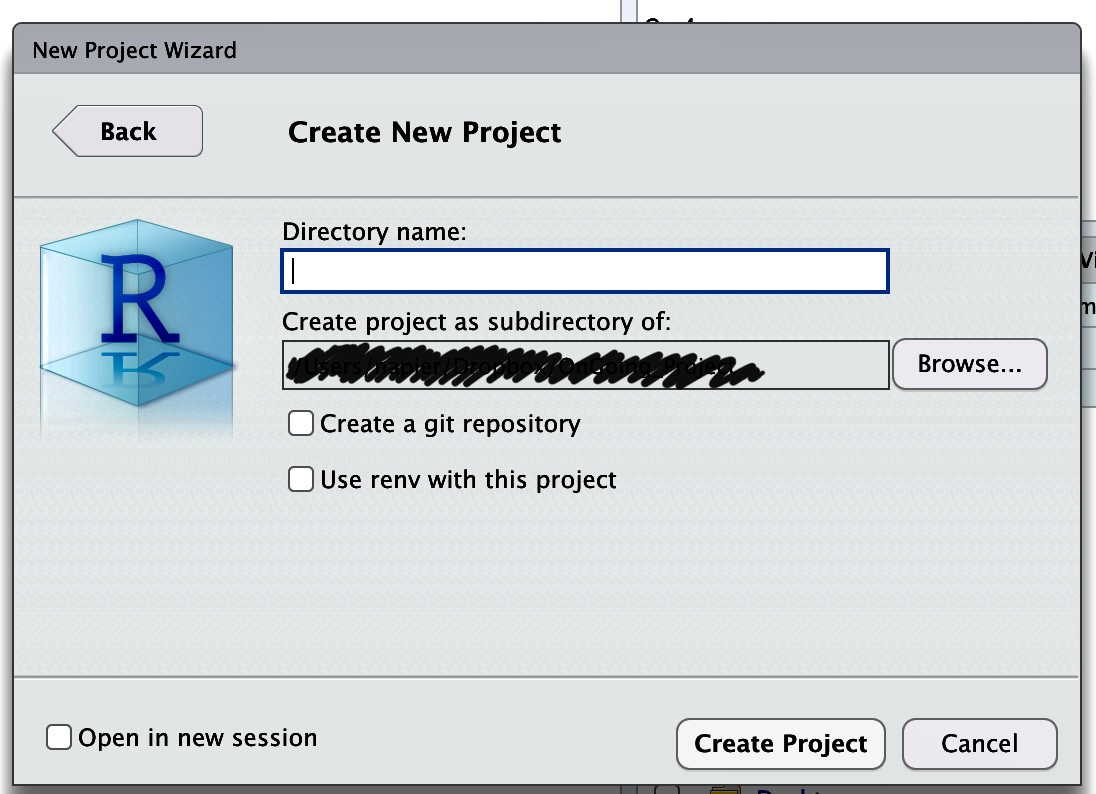
\includegraphics[keepaspectratio,width=0.65\linewidth]{../images/03_introR/Screen5.png}
    \caption{プロジェクトを作る場所を選ぶ}
    \label{fig::05_05}
\end{figure}

図\ref{fig::05_05}には\verb|New Directory > New Project|と進んだ次のウィンドウを示しています。黒く塗りつぶしているところは私の個人的なPC環境の内容が反映されるので誤魔化しているのですが，みなさんの環境にあった場所(DocumentとかDesktopと言った場所)を選び，上の空白になっているところに新しいプロジェクト名(たとえば\text{toukei}など\footnote{半角英数のみで作るべきです。})を入力してOKとします。するとしばらくすると，画面が変わるはずです。一見同じ状態のようにも見えますが，実はところどころ違いがあります。気がつきましたか？
\begin{figure}[ht]
    \centering
    
\includegraphics[keepaspectratio,width=0.8\linewidth]{../images/03_introR/Screen6.png}
    \caption{プロジェクトで開いている場合}
    \label{fig::05_06}
\end{figure}
図\ref{fig::05_06}にはプロジェクトを開いている時のRStudio画面を示しています。赤く丸で囲っているところが，プロジェクトを開いていない時との違いがある箇所です\footnote{MacOSの例なのでWindows版では上のバーのところなど，違いもあります。}。これをみると，コンソールペインやFileペインの場所に，今指定したフォルダの位置が示されていることがわかります\footnote{この例では\verb|C:\Users\napier\Desktop\toukei|です。napierは私のPCの名前，toukeiはプロジェクト名です。}。このプロジェクトが開いているフォルダに移動していることが重要で，このフォルダの中が今作業している場所として認識されるので，このフォルダの中にあるファイルにはファイル名だけでアクセスできるようになります。プロジェクトが違ったり，プロジェクトの起動をしていなかったりすると，作業している場所\footnote{ワーキングディレクトリといいます。詳しくは付録の\ref{setLocation}を参照。}が変わりますので，注意が必要です\footnote{実際に授業をしていて，ファイルへのアクセスエラーで相談を受ける原因第2位です。第1位はファイルエンコードの問題です。}。

\subsection{エラーはヒントです。怖がらないで}
\label{DontBeAfraid}
以下ではみなさん自身でRコードを書いていくのですが，誰しも，間違いなく，エラーに遭遇します。
エラーはムカつきますし，理由がわかりませんし，何書いているかわからん！ってなりますよね。

でも，エラーはヒントなのです。ここでこういうエラーが生じましたよ，というヒントをくれているし，それに対応しさえすればちゃんと動いてくれます。
プログラムは思った通りに動くのではなく，書いた通りに動くのです。
ですから，赤字で何か出てきた場合はどういうエラーなのかを読み取るようにしましょう。何行目の，どの部分で生じたエラーかが別れば，対応の仕方がわかります。

最初のうちはエラーの読み方もわからないと思います。そういう時は遠慮なく質問してください。ただし質問する時に「エラーが出て動きません」とだけ言われても困ります。エラー情報がないと私も対応できませんから。
「何行目を実行したら，これこれこういうエラーが出て動きません」と言われると，対応できます。怖がらずに進めていきましょう。



\section{Rの基本操作}
ではこのプロジェクトの中で、演習を進めていきましょう。
先ほどと同じように，\verb|File > New File|から \verb|R Script|と進んで新しいスクリプトファイルを開きます。

今から色々書いていきますが，これを記録しておくには，ファイルを保存する必要があります。\verb|File > Save|と進むと保存できますので，ファイル名をつけて保存します。拡張子\footnote{拡張子については，付録\ref{suffix}を参照のこと。}は\texttt{.R}にしておきましょう(小文字の\texttt{.r}でも結構です)。とくに思いつかなければ，\texttt{Lesson01.R}とでもしておいてください。

\subsection{関数の利用}
先ほど，\texttt{sqrt(16)}という関数の例をみました。この\texttt{sqrt}関数はスクェアルート，つまり平方根を求めろというものです。何の平方根を求めるか，というと16という数字の平方根ですので，実行すると4という答えが返ってくるわけです。

このように，関数名で命令を指定し，その対象は小かっこ\verb|()|で囲って渡すというやり方をします。$f(x)$ということですね。括弧の中に入るものは\keyterm{引数}{ひきすう}{argument}といい，今回のように目的となる数字を渡すこともありますが，そのほか関数を動かす上でのオプションを指定することもあります。また，1つの引数だけではなく，複数の数字を渡したり，複数のオプションを指定することもあります。

たとえば関数がどのように動くか知りたいという時，ヘルプを開くのも関数で行います。\texttt{code:\ref{code:05_02}}を実行すると，Helpペインにその説明が出てくるので確認してみてください。
\begin{lstlisting}[language=c++,label={code:05_02},caption={ヘルプのコード}]
	# ヘルプも関数
	help(sqrt)
\end{lstlisting}
\subsection{パッケージの利用}
\label{HowToUseRpackage}
Rでは関数を使ってさまざまな計算をこなします。Rをインストールした段階でも，簡単な統計計算は十分できるようになっています。ですが，より専門的な分析やより高機能な情報処理をしようとするならば，\keyterm{パッケージ}{ぱっけーじ}{package}を利用することになります。たとえば，包丁一本で料理をするのは大変ですよね。包丁は確かに切ったり，皮を剥いたり，削ったり・・・と色々できることはできるのですが，皮を剥くのはピーラーで，細かく削るのはフードプロセッサーで，といった便利グッズを使えばもっと楽です。この「便利グッズ」がRでいうところのパッケージです。

Rは豊富なパッケージが利用できることがその特徴で\footnote{本講執筆時点(2021/02/05)で289,680件のパッケージがCRANに登録されています。それ以外にも無数のパッケージがGitHubなどで公開されています。}，パッケージはCRANを通じて世界に公開されています。RStudioのパッケージペインを開くと\texttt{install}と\texttt{update}というボタンがありますが，\texttt{install}ボタンを押すと何のパッケージをとってくるか，入力できるようになります(図\ref{fig::usingR_pkgInstall})\footnote{出てくるボックスに示された，``Install From''が「どこからとってくるか」を示している欄になりますが，これはCRANが自動的に選択されているので変更する必要はありません。}。``Packages''とあるところに必要なパッケージ名を入力すると，自動的にCRANにアクセスしてダウンロードが始まります。パッケージのインストールとダウンロードはその環境下では一度実行するだけで結構です。パッケージというのは関数群であり，関数を記載したファイルのダウンロードが終われば適切な場所(Library)に保存されます。

ただ，ダウンロードしただけではすぐにその関数が使えるようになりません。ダウンロード後は，必要に応じて\texttt{library}関数でパッケージを呼び出してやると，パッケージに含まれる関数が使えるようになります。購入したものを装備するかどうかは別，ということを頭の片隅に置いておいてください\footnote{と同時に，同じパッケージを何度もダウンロードする必要はないということです。もっとも，Rのバージョンが上がるとか，違う環境で実行する場合は再ダウンロードが必要なこともあります。}。
また，パッケージの中には関係するパッケージを一まとめにしたパッケージというのもあります。インターネットへのアクセスは必要ですが，優れたパッケージを無償で入手できますので，便利なものをいくつか決めていれとくと良いでしょう。本講義で必要なパッケージは随時指定しますが，ひとまずは\texttt{tidyverse}パッケージ\citep{tidyverse}を入れておきましょう\footnote{この\texttt{tidyverse}パッケージは，実はパッケージのパッケージですので，これをインストールしようとすると関連するその他のパッケージを次々と自動的に呼び出して環境を整えてくれます。初回は少し時間がかかりますが，気長に待ちましょう。大学のPC室や計算機サーバなどには，すでにインストールが終わっているのでその作業は必要ありません。}。

\begin{figure}[ht]
    \centering
    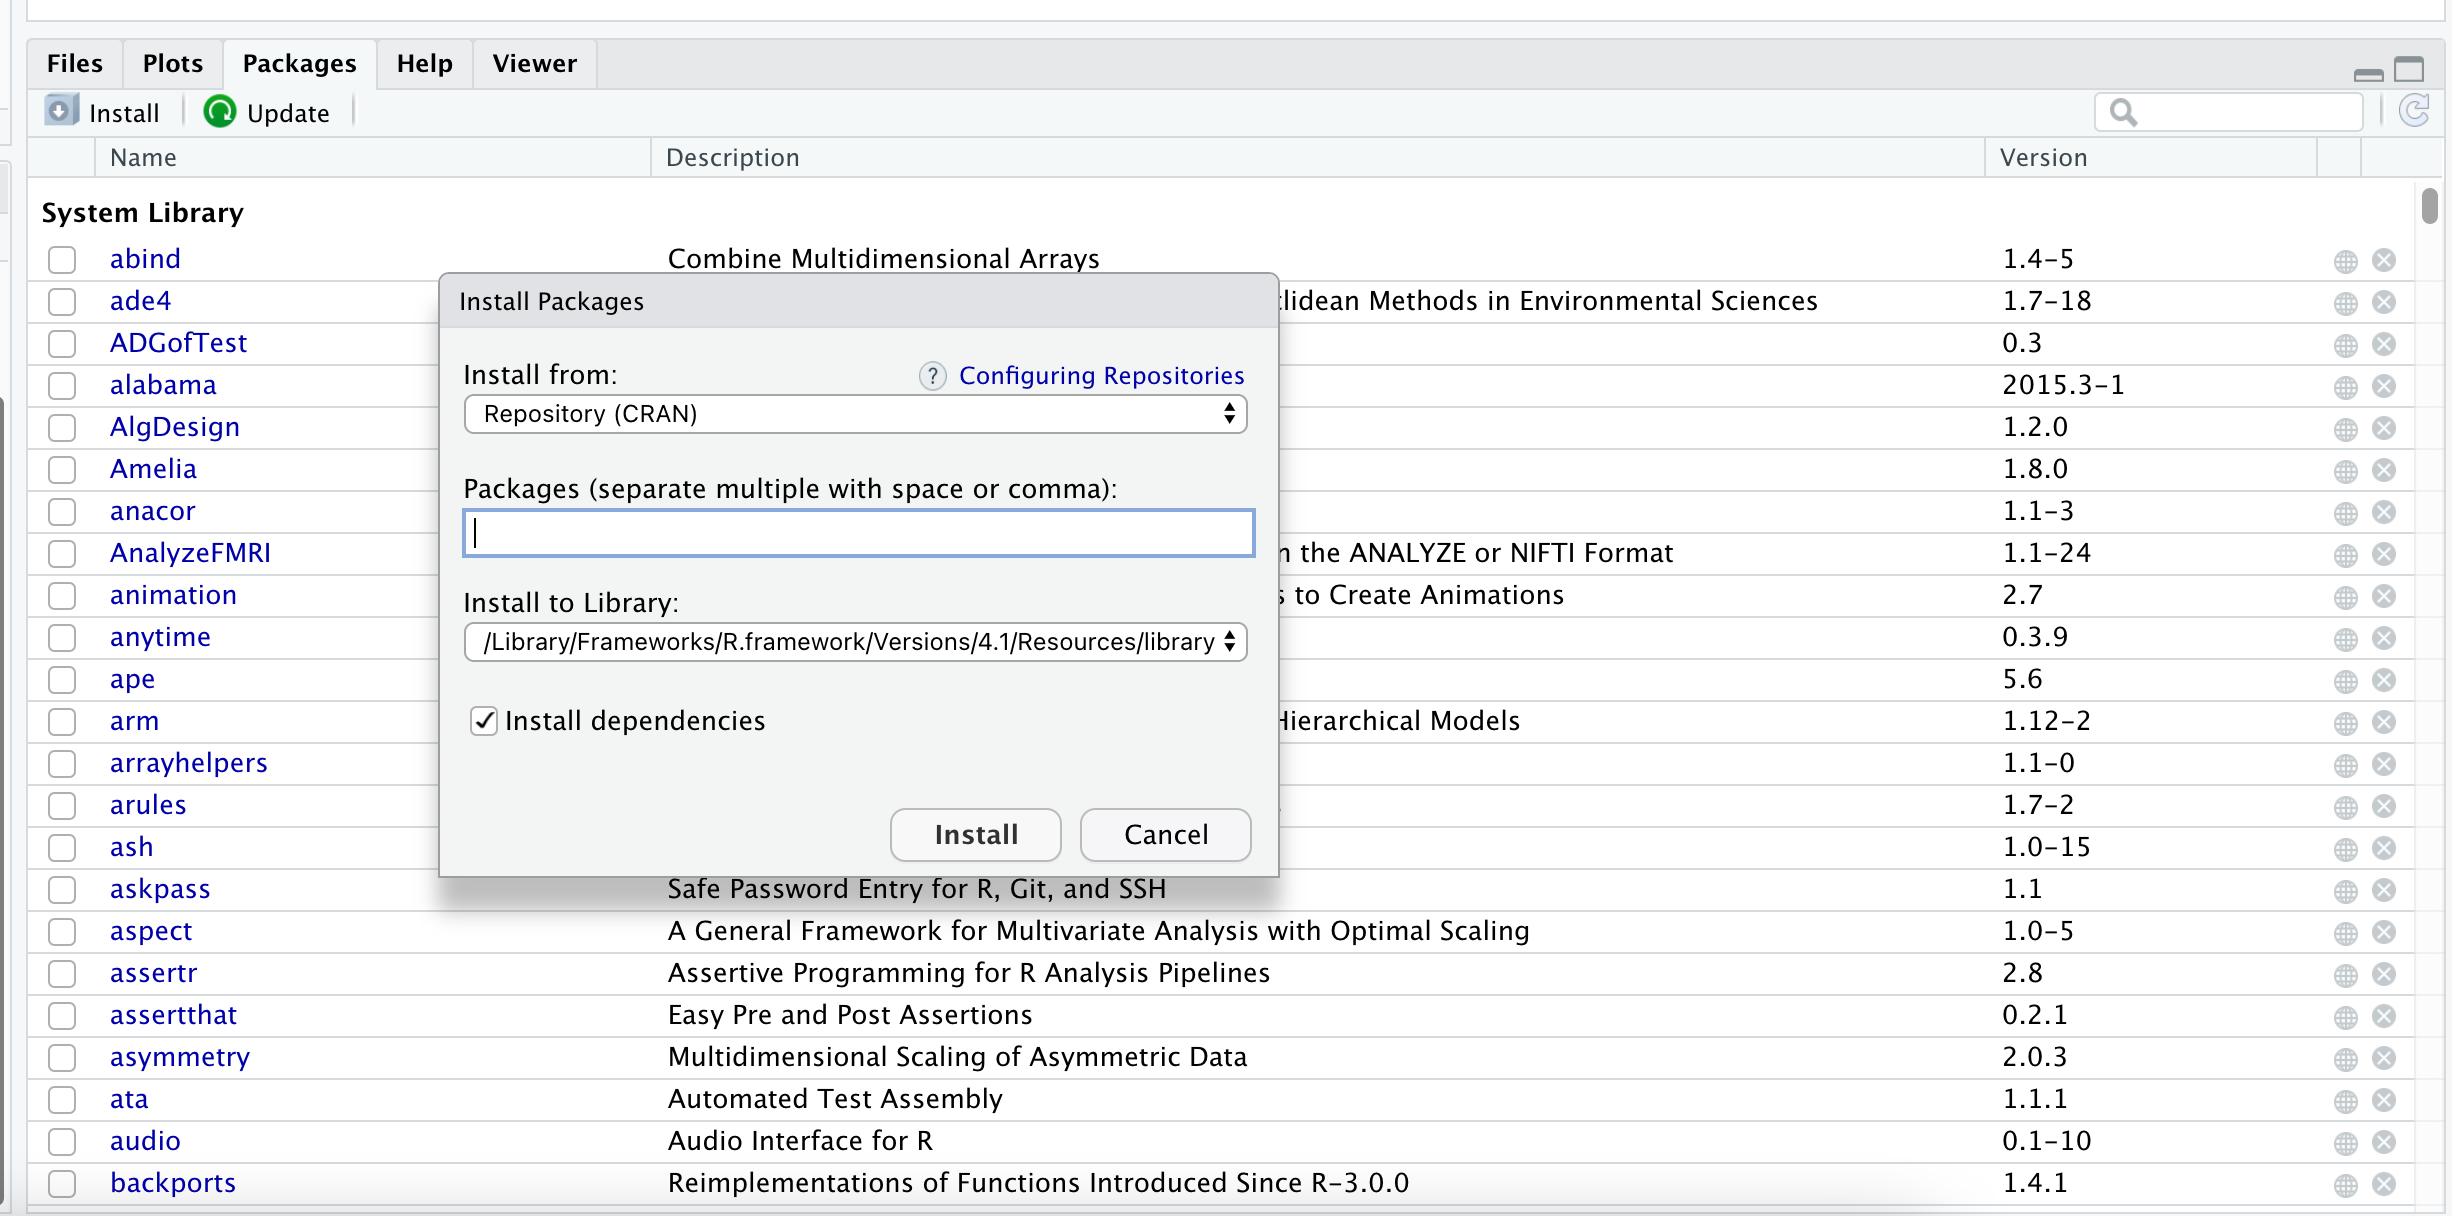
\includegraphics[keepaspectratio,width=0.8\linewidth]{../images/04_usingR/screen16.png}
    \caption{PackageタブからInstallをクリック}
    \label{fig::usingR_pkgInstall}
\end{figure}


このインストールは，RStudioのパッケージペインからも実行できますが，\texttt{code:\ref{code:05_02b}}のようにコードを使って実行することも可能です。
\begin{lstlisting}[language=c++,label={code:05_02b},caption={コードからインストールする}]
install.packages("tidyverse")
\end{lstlisting}

% \begin{tcolorbox}[title=パッケージのインストール先,fonttitle=\gtfamily\sffamily\bfseries,colframe=blue,colback=blue!3!]
% 　ここでエラーに遭遇して「パッケージがインストールできない！」となることがあります。Windowsユーザがよく直面します。

% 　原因はいくつか考えられますが，ほとんどが文字化けに起因したものです。
% 　パッケージといっても電子データ，ファイルで提供されるものであり，インストーリとはインターネットからファイルをダウンロードしてくるところから始まります。
% ダウンロードしてきた情報は手元のPCにファイルとして保存することになりますが，ここで「保存先に\textbf{書き込み権限がない}」ことでエラーになる，というのが第一の問題です。エラーメッセージの中に\verb|'lib = "C:/Program Files/R/R-4.1.1/library"' is not writable|などとあれば(is not writable=書けないよ)，このエラーです。その場合は，R/RStudioを\underline{管理人権限で実行する}必要があります。アイコンを右クリックして，サブメニューから管理人として実行を選びましょう。

% 　第二の問題は，書き込む先のフォルダ名に起因するものです。エラーメッセージの中に\verb|ディレクトリ'C:\Users\XXXX\OneDrive\?????'を作成できません|とあれば，この問題です。ここでXXXXと書いてあるのはみなさんのPC名，\verb|????|が文字化けの箇所です。ユーザ名として2バイト文字=全角文字を使っているWindowsユーザだけがこのエラーに遭遇します。理由はWindowsの不親切設計，一貫しないOSデザインのせいです。パソコンを買ってきたら自分の名前を漢字で入力したいですよね。漢字でユーザを作るとそれで動いてくれたらいいのですが，なぜかWindowsはここで文字コードのエラーを起こすのです。他のOSであれば，文字コードはUTF-8に統一されているのでこの問題は生じません。
% 　解決策としては，半角英数文字のユーザを作り直し，そのユーザでRのインストールをやり直すか，パッケージをダウンロードする先のフォルダをこちらで指定してやるかの二択です。
% 　後者の方法は，まずインストール先がどこになっているかを確認する必要があります。Rのコンソールに\verb|.libPaths()|と入力してみてください。ここで表示されるのが，ライブラリへのパス，つまりパッケージが保存される場所です。もしここに全角文字があれば，エラーになります。
% 　そこでまず，全角文字を含まない場所にパッケージをインストールするフォルダを用意します。PCのCドライブ直下に作るのが良いでしょう。たとえば\verb|C:/Rlibrary|のようなフォルダを準備します。
% 次にRで，この関数を使って，\verb|.libPaths("C:/Rlibrary")|のように，先ほど作ったフォルダを指定します。
% これでインストール先が変わるので問題なくインストールできるでしょう。

% 　最後に1つ注意を。Rを再起動するたびに\verb|.libPaths()|がリセットされるケースがあります。これはRの環境変数が設定されているからで，これを修正するには\verb|.Rprofile|ファイルを作るとか，コマンドプロンプトやコントロールパネルから環境変数\verb|R_LIBS_USER|を設定する必要があります。
% \end{tcolorbox}


\subsection{オブジェクトの利用}
Rで扱う変数、関数、データセットなどにはすべて，名前がついています。なまえがついた「それ」のことをオブジェクトと呼びます\footnote{適当な日本語訳がありません。objectはもの，対象という抽象的な意味なので，カタカナでオブジェクトとするしかないのです。}。\texttt{code:\ref{code:05_03}}を書いてみてください。
\begin{lstlisting}[language=c++,label={code:05_03},caption={オブジェクトに代入}]
	# オブジェクト
	A <- 2
	B <- 3
	A + B
	A
\end{lstlisting}
\begin{description}
    \item[1行目] コメント
    \item[2行目] Aと名付けたものに数字の2を代入する。代入の記号は小なり(\verb|<|)とハイフン(\verb|-|)の二文字でできていて，矢印記号$\leftarrow$を表しています。RStudioの機能で，Macの場合はoptionとマイナス記号，Windowsの場合はAltキーとマイナスを同時に押すと入力できます。。
    \item[3行目] Bと名付けたものに数字の3を代入しています。
    \item[4行目] オブジェクトAとオブジェクトBを足し合わせています。
    \item[5行目] オブジェクトAの中身を表示させろ(中身はなんだっけ)，という意味です。
\end{description}

実行結果は\texttt{Rの出力\ref{RS:out05_02}}のようになるでしょう。
\begin{Rscreen}{オブジェクトに代入する}{out05_02}
    \begin{verbatim}
> # オブジェクト
> A <- 2
> B <- 3
> A + B
[1] 5
> A 
[1] 2
\end{verbatim}
\end{Rscreen}
一行目は当然なんの回答もありませんが，2，3行目を実行してもすぐに次のプロンプト(\verb|>|)がでて指示待ちになります。これは「代入しろ」といわれたから代入したのであって，とくに反応を求めてないからです。次の4行目になって初めて足し算をせよ、と言われたのでその結果が5である，と返答しています。また，5行目はAとだけ入力されました。このように指示待ちの時にそのオブジェクト名を入れると，その中身をすべて表示してくれます。今回は2がはいっているので，2ですよ，と答えてくれています。

このようにオブジェクト名だけで計算を進めることが可能です。オブジェクト名はなんでもいいのですが，\texttt{TRUE, FALSE, NA}などRが特別な意味を持たせている言葉や，\texttt{pi}などの数学的意味がある言葉は予約語といって既に使われているので，そのままの方がいいでしょう。かといって，A, B,Cといった無味乾燥な記号でもわかりにくいので，その時々に応じて任意の名前をつけてあげてください。

ちなみにこの「オブジェクトに代入」は基本的に上書きされるというルールです。さきほどのコードに続いて\texttt{code:\ref{code:05_04}}を書いてみてください。
\begin{lstlisting}[language=c++,label={code:05_04},caption={オブジェクトは上書き}]
A <- 4
A + B
\end{lstlisting}
今度は結果として7が表示されたと思います。先ほどはAに2を代入せよといい，そのあとでAに4を代入せよと命じたので，いまAは4に上書きされています\footnote{オブジェクトの中に何が入っているかは，Environmentタブをみるとわかることがあります。今見ると，Aに4，Bに3が入っていることが示されているでしょう。}。この基本的に上書きされる，ということはよく注意しておいてください。というのも，これから長いコードを書くことがあったときに，部分的に実行を繰り返すと上書きに上書きを繰り返すこともあり得るからです。そうすると，ある時うまくいったけど，次に同じことをしようとしたらうまくいかなかった，ということにもなりかねません。くどいようですが記録は再現性の担保のためにやっているわけですから，一時的な記憶やたまたまうまくいった例に依存しては困ります。環境が空っぽの状態，クリアな状態で一行目から順に走らせて，何度やっても同じ答えが出るようにしましょう。

環境をクリアにするには，Environmentタブのバーにある箒のアイコンをクリックします。これでRの頭の中が空っぽになります。あるいは\texttt{rm(list=ls())}というコードを実行するとクリアされます。スクリプトの一行目にこれを書いておくことをお勧めします。

また，Rは終了すると，それまでの作業を保存しますから，同じプロジェクトをもう一度開くと以前の記憶が蘇ります。これが便利なのですが実は少し厄介で，学生さんが「自分の環境ではできた」といっても私の手元で再現できない(からレポートやり直し)ということがあります。きっと記録されているスクリプトの外で，なんらかの作業がなされているのです。清書できたスクリプトは，Rの頭の中を空っぽにしてから再チェックすると良いでしょう。また，\verb|Tools > Global Option|から，Workspaceの``Restore .RData into workspace at a startup''(起動時に.RDataからワークスペースの情報を復元する)のチェックを外し，``Save workspace to .RData on exit''(終了時に.RDataにワークスペースの情報を保存する)を``never''(絶対そんなことしない)にしておくことで，いつでもクリーンな環境から始められます(図\ref{fig::05_07})。

\begin{figure}[ht]
    \centering
    
\includegraphics[keepaspectratio,width=0.65\linewidth]{../images/03_introR/Screen7.png}
    \caption{クリーンな環境をいつでも保つための設定}
    \label{fig::05_07}
\end{figure}

\subsubsection{オブジェクトの型1・ベクトル}
\texttt{code:\ref{code:05_05}}を実行してみましょう。
\begin{lstlisting}[language=c++,label={code:05_05},caption={ベクトル処理}]
	obj1 <- 1:10
	obj1 + 2
	obj2 <- c(2,3,4,1,2,3,4,5,6,7)
	obj1 + obj2
\end{lstlisting}

\begin{description}
    \item[1行目] \texttt{obj1}オブジェクトに``1:10''を代入
    \item[2行目] \texttt{obj1}オブジェクトに2を加える
    \item[3行目] \texttt{obj2}オブジェクトに``c(2,3,4,1,2,3,4,5,6,7)''を代入
    \item[4行目] \texttt{obj1}オブジェクトに\texttt{obj2}オブジェクトを加える
\end{description}

一行目で代入している``1:10'' はR独特の表記法で，コロンで繋いだ数字は連続した数字を意味します。ここでは1から10までの連続した数字，すなわち$1,2,3,4,5,6,7,8,9,10$です。このように数字のセットを一度に扱うことができます。このオブジェクトに2を加えるというのは，各要素に2を加えることと同じですので，そのような結果が出力されていますよね。
また三行目で代入しているのは$2,3,4,1,2,3,4,5,6,7$という数字列です。これを\texttt{c}関数で括っています。この\texttt{c}は一文字ですが関数で\footnote{combineやconcatenateの略語と言われています。}，数字をセットにするという働きをします。そして四行目で，対応する各要素を足し合わせるという計算を行っています。

このように，数字をセットで扱うことができるのが電卓とは違うところです。統計ではたくさんのデータを扱うわけですから，この機能は基本中の基本になります。ちなみに，数字のセットのことは数学でベクトルというのでした。今回のオブジェクトは数字をベクトルとして保管していることになります。

\subsubsection{オブジェクトの型2・リスト}
データセットは数字だけではなく，文字列などを含むことがあります。そうした対象をまとめて扱うのが\keyterm{リスト}{りすと}{list}という形式です。つづいて\texttt{code:\ref{code:05_06}}を実行してみましょう。
\begin{lstlisting}[language=c++,label={code:05_06},caption={リスト型}]
	obj3 <- list(
		name = c("Taro", "Hanako", "Ken"),
		gender = c("male", "female", "male"),
		height = c(170,160),
		weight = 55
	)
	obj3
	obj3$name
\end{lstlisting}
\begin{description}
    \item[1行目] \texttt{obj3}オブジェクトに代入するのは\texttt{list}であることを，\texttt{list}関数を使って明示しています。この関数の中身は複数行にわたり，括弧が閉じられるのは6行目になりますので，そこまでで1つの命令文だということになります。
    \item[2行目] nameという名前のついたベクトルを作ります。
    \item[3行目] genderという名前のついたベクトルを作ります。
    \item[4行目] heightという名前のついたベクトルを作ります。
    \item[5行目] weightという名前のついたベクトルを作ります。要素が1つでも，要素1のベクトルとRは解釈します。
    \item[6行目] 1行目から続く\texttt{list}関数の終わり。リストの中に含まれるベクトルは間まで区切られていること，対応する括弧がきちんと閉じられていること，が重要です。
    \item[7行目] オブジェクトの中身はなあに，ということで中身を表示させています。
    \item[8行目] \texttt{obj3}オブジェクトのname要素だけにアクセスしてみました(要素を見せて，と命じている)。
\end{description}

出力された画面を見て，何が起きているかを確認してみてください。コードの2から6行目に当たるところでは，コンソールの左端が\verb|>|ではなく\verb|+|になっていると思います。これは前の行から続いて入力されている，つまり入力がまだ終わっていないことを意味する記号になっています。また7,8行目については，表示させる指示をしているので，その結果が返ってきているはずです。

このように，名前(文字列)や性別(名義尺度水準)，身長や体重(比率尺度水準/量的変数)などをひとまとめにして\texttt{obj3}というオブジェクトに保管する，ということができています。このオブジェクトのある変数だけ参照したい，というときは，オブジェクト名の背後にドルマーク(\verb|$|)をつけて繋げます。RStudioで入力してる時は，\verb|obj3$|と書いただけで「中身はこれですが」という候補のリストが示されたと思います。このように入力補完をしてくれるのもRStudioのいいところです。

ところでこれがデータセットだとすると奇妙ですね。名前や性別は3つありますが，身長は2つ，体重は1つしかデータがありません。普通こんなことはなくて，1つのケースについて複数の変数があるので，縦に個体$\times$横に変数の長方形型をしているデータセットが一般的になるはずです。リスト形式は各要素の長さに関係なく，なんでもまとめて置けるので便利なのですが，データ分析においては長方形であるという形の制約があって良いはずです。この制約を持ったリスト形式のことを\keyterm{データフレーム}{でーたふれーむ}{data.frame}型と言いいます。
\subsubsection{オブジェクトの型3・データフレーム型}
データフレーム型にするには，\texttt{data.frame}という関数を使います。\texttt{code:\ref{code:05_07}}を実行してください。
\begin{lstlisting}[language=c++,label={code:05_07},caption={データフレーム型}]
	df <- data.frame(
		name = c("Taro", "Hanako", "Ken"),
		gender = c("male", "female", "male"),
		height = c(170,160,155),
		weight = c(55,60,43)
	)
	df
	df$name
\end{lstlisting}
\begin{description}
    \item[1行目] \texttt{df}オブジェクトに代入するのは\texttt{data.frame}であることを，\texttt{data.frame}関数を使って明示しています。
    \item[2行目] nameという名前のついたベクトルを作ります。
    \item[3行目] genderという名前のついたベクトルを作ります。
    \item[4行目] heightという名前のついたベクトルを作ります。要素数を合わせます。
    \item[5行目] weightという名前のついたベクトルを作ります。要素数を合わせます。
    \item[6行目] 1行目から続く\texttt{data.frame}関数の終わり。ここに含まれるベクトルは間まで区切られていること，対応する括弧がきちんと閉じられていること，が重要です。
    \item[7行目] オブジェクトの中身はなあに，ということで中身を表示させています。
    \item[8行目] \texttt{df}オブジェクトのname要素だけにアクセスしてみました(要素を見せて，と命じている)。
\end{description}
コンソールには\texttt{Rの出力\ref{RS:out05_03}}のように表されていると思います。
\begin{Rscreen}{オブジェクトに代入する}{out05_03}
    \begin{verbatim}
> df <- data.frame(
	+     name = c("Taro", "Hanako", "Ken"),
	+     gender = c("male", "female", "male"),
	+     height = c(170,160,155),
	+     weight = c(55,60,43)
	+ )
> df
	name gender height weight
1   Taro   male    170     55
2 Hanako female    160     60
3    Ken   male    155     43
> df$name
[1] "Taro"   "Hanako" "Ken"
\end{verbatim}
\end{Rscreen}
このオブジェクト，\texttt{df}の出力を見るとわかるように，行に個人，列に変数の長方形方になっています。変数にアクセスする時は，list型の時と同じようにオブジェクト名の背後に\verb|$|をつけて，\verb|df$name|のようにします。

今回はひとまずデータを作るために，各ケースの値を入力して行ってもらいましたが，実際に統計解析をする時は表計算ソフトで素データを入力し，ファイルからRにデータを読み込むことが一般的です。これについては第\ref{m04_usingR}講で説明します。


\section{再現性のある研究実践へ}
\label{reproducibility}

さて，これで演習の第一段階は終了です。
Rのスクリプトを書いてみて，いかがだったでしょうか。思った通りに動かない，とイライラしたひともいるかもしれません。その通り，\textbf{コードは思った通りに動くのではなく，書いた通りに動く}のです。正しく指示し，正しい答えを得るために，実行記録が残るということは科学的営みとして重要なことなのです。

今後，みなさんはパソコンを使って文章(レポートや論文)を作成するという機会が増えてくることは間違いありません。文字を入力するだけであればスマートフォンでもいいですが，レイアウトを整えるためにはパソコンが必要になってきます。文章だけでなく，図表も作成することになりますし，図表を作るのに必要な統計的データの整理，分析もパソコンを使って行います。とくに図表や統計分析は，プログラムを書いて行うことになります。機械は0と1の羅列で情報処理をしますが，その文字列を人間が考えるのは大変です。機械にやって欲しい操作，計算を人間がわかる言葉で書いたものをプログラムと言います。機械と人間を繋ぐ言語だと思ってください。この言語には色々な種類がありますが，基本的に統計環境Rという言語を使えるようになってください\footnote{2023年度も，専修大学心理学科で公式に使う統計環境になっています。}。

計算だけでなく図表を書くのも，プログラミングすることになります。なぜそんな面倒なことをするのでしょう？ 表計算ソフトを使うと，誰でもマウスでカチカチっとすれば簡単にグラフが作れるのに，と思った人もいるかもしれません。その答えは端的にいうと，そのやり方だと記録が残らないからです。同じデータに同じプログラムをあてがえば，別の計算機上でも結果が同じになります。この誰がどこでやっても同じ結果になる，というのが科学の営みとして重要なことであるのは第\ref{m01_introduction}講で説明した通りです。また，教員と研究指導のやりとりをする上でも，プログラムに書き起こされていることは利点があります。マウスでの動きを口頭で説明するのは難しいですね。さらに自分がどういう設定・環境で実行したかを完全に意識していない場合，「なんだかわからないけど，カチカチやっているうちにこの結果が出ました」ということにもなりかねません。そういう報告を受けた教員の気持ちも想像してみてください。指導のしようがありません。

プログラムで実行するというのはすなわち，何をどのように操作するのかを書き下すことでもあります。すごく複雑な統計処理も，中身は1つ1つの「計算」の積み重ねです。何がどのように積み重なっているかをしっかり理解しなければ書けません。逆に言えば，書いてあるものを見ればどのように組み立て，どのような実行をしているのかがわかります。うまくいかないプログラム，つまりエラーがおきるプログラムであっても，プログラムされたコード(スクリプトとも言います)を見せてもらえれば，どこにエラーが生じているかを明らかにできます。研究の実践とその成果が「動作」ではなく「指示書」として記録に残ることは，研究の再現性を高めるためにも重要な営みなのです。

教育や学習の上でも利点はあります。プログラムを書くときに必要なのはこのアルゴリズム的思考，すなわち目標に向かうための必要な手続きを1つ1つ特定し，順序立てて実行していくという考え方です。お料理のように，「玉子焼き」というゴールに到達するために「卵を取る」「卵を割る」「卵をかき混ぜる」「フライパンを温める」...といった各手続きを順序立てて実行できなければなりません。これから先，統計の話が複雑になってくると，わからない！と音を上げたくなることが出てくるかもしれません。そんなときは(たっぷり休憩して心身ともに元気な状態で落ち着いて)見直すことで，どこからどこまで理解していて，どこから理解できていないのか，確認できます。プログラムのエラーの場合，どこからどこまでが正常に動いていて，どこから計算がおかしくなるのかを見ることができるのです。諦めなければ，確実に積み重ね，前進できます。エラーが出ると言いましたが，エラーはたいていの場合エラーメッセージとともに明らかになります。このメッセージをよく読めば，解決のいとぐちが掴めるのです。わからなければエラーメッセージとともに，教員に相談してください。どこでどのようなエラーが出たかをじっくり確認すれば，何が間違いで何がわかっていなかったのかがわかるというものです。エラーを1つ1つ無くしていき，うまく動くプログラムが書けたときは嬉しいものですよ。

最後に，プログラムを含めて記録の取れる研究実践について少しだけ説明しておきます。科学は「自分だけがわかっている」という私秘性を排除した公共的な営みである，ということはすでにお話しした通りです。個々人の興味関心によって研究を積み重ねていくのですが，研究の結果明らかになったことはオープンな議論の場に出すべきです。なぜなら，自分が知りたいと思って始めた研究について，他の人から自分では気づかなかった問題点を指摘してもらえるかもしれないし，もっとおもしろいテーマに展開できるかもしれない，あるいは他の人と一緒に研究しようということになるかもしれないからです\footnote{間違いを指摘されたら恥ずかしい，などと思ってはいけません。間違いは正せばいいだけですし，間違いが直るとより良いものになっていくだけだからです。小中高の学校教育とは違って，正解がある問題を考えているわけではないので，教員はもちろん周りの人の目を気にする必要はまったくありません。そんなことでからかう人がいないのが大学という界隈の楽しいところです。}。自分の研究も他人の研究の成果を踏まえて，あるいはそこからインスパイアされて進めることになりますが，この研究のスタートとなるこれまでの成果に間違いや嘘が含まれていては困りますね。人間を対象にした研究の場合は，間違いや嘘がまったく含まれていなくても完全に同じ状況や同じ対象に研究するというのが難しいので，先行研究の結果が再現できないという問題があります\footnote{実際，社会心理学の教科書に載っているような研究は再現率が30\%しかない，という批判もあります。詳しくは\citet{Ikeda2016}などを読んでください。}。

そこで，何をどのように研究したか，どういうデータをとってどのように分析したか，ということを事細かく記録しておく必要があります。最近では，研究を始める前に事前にどのような研究計画で進めていくかを公開し\footnote{研究をする前に計画だけの論文をチェックしてもらう方法もあります。プレレジストレーション，略してプレレジと言います。}，とったデータや分析プログラムも公開するということが行われています。こうした研究計画やデータ，プログラムの公開はOpen Science Frameworkというウェブサイト\footnote{\url{https://osf.io/}}が今最もよく利用されています。ここでファイルを共有すると，いつどのようなファイルが置かれたか，どのように更新されたかという記録が残るので，記録の改竄などを疑われるような懸念がなくなるという利点もあります。

皆さんも，ごく初心者とは言え心理学という科学の営みをするメンバーの一人になったわけですから，自分の記録やファイルを管理し，公開するという意識を持って取り組むようにしてください。

\section{課題}
\paragraph{自分の電子機器のスペックを調べる}
皆さんが使っているパソコンの，CPUのメーカー，型版はどういったものですか。一次記憶装置はどれぐらいの容量がありますか。二次記憶装置の容量はどうですか。いま二次記憶装置の空き容量はどれぐらいですか。調べて回答してください。
\paragraph{自分のファイルの場所を調べる}
同じくパソコンのユーザ名は何になっていますか。また何か適当なファイルを作り，どこかに保存し，「どこにどのようなファイル名で保存したか」を報告してください。拡張子をつけることを忘れずに。
\paragraph{Rで遊んでみよう}
今日実行したRのコードはごく簡単な計算ばかりです。数字を色々書き換えて遊んでみましょう！
\end{document}

